\documentclass[12pt,a4paper]{article}

% ===================== Packages =====================
\usepackage[utf8]{inputenc}
\usepackage[T1]{fontenc}
\usepackage{graphicx}
\usepackage{geometry}
\usepackage{amsmath,amsfonts,amssymb}
\usepackage{times}
\usepackage{float}
\usepackage{enumitem}
\usepackage{hyperref}
\usepackage{caption}
\usepackage{booktabs}

\graphicspath{{.}{./}{../}}

\geometry{margin=1in}

% ===================== Document =====================
\begin{document}

% ===================== Title Page =====================
\begin{titlepage}
    \centering
    
    % College Logo
    
\includegraphics[width=0.3\textwidth]{iiit_kalyani_logo.png}\\[1cm]
    
    {\Large \textbf{Indian Institute of Information Technology Kalyani}}\\[1.5cm]
    
    {\Large \textsc{Major Project Report}}\\[0.8cm]
    
    \rule{\linewidth}{0.5mm} \\[0.4cm]
    {\huge \textbf{Complete Plotting for a COVID-19 Based Epidemiological Model}} \\[0.2cm]
    \rule{\linewidth}{0.5mm} \\[1.5cm]
    
    \begin{minipage}{0.45\textwidth}
        \begin{flushleft} \large
            \emph{Submitted by:}\\[0.3cm]
            \textbf{Shashi Prakash Yadav} \\ {\small [CSE/23096/1144]}\\[0.2cm]
            \textbf{Mohd. Usham} \\ {\small [ECE/23125/1173]}\\[0.2cm]
            \textbf{Rishabh Kumar} \\ {\small [ECE/23133/1181]}\\[0.2cm]
            \textbf{Ritik Aryan} \\ {\small [ECE/23134/1184]}
        \end{flushleft}
    \end{minipage}
    \hfill
    \begin{minipage}{0.45\textwidth}
        \begin{flushright} \large
            \emph{Project Mentor:} \\
            \textbf{Dr. Sudeshna Mondal}
        \end{flushright}
    \end{minipage}
    
    \vfill
    
    {\large \today}
\end{titlepage}

% ===================== Certificate =====================

\newpage

% ===================== Declaration =====================
\section*{Declaration}
We hereby declare that the work presented in this project report is an authentic record of our own work carried out under the guidance of our mentor. The work has not been submitted to any other university or institute for the award of any degree.

\vspace{2cm}
\noindent
Shashi Prakash Yadav \\
Mohd. Usham \\
Rishabh Kumar \\
Ritik Aryan

\newpage

% ===================== Abstract =====================
\section*{Abstract}
The COVID-19 pandemic has highlighted the importance of mathematical modeling in understanding disease transmission and evaluating control strategies. In this project, we study a compartmental epidemiological model incorporating susceptible, exposed, quarantined, infected, and recovered populations. Using parameters motivated by real-world data, we analyze the basic reproduction number, stability of equilibrium points, sensitivity of parameters, and visualize system dynamics through extensive plotting. The results provide insights into the role of quarantine and governmental intervention measures in mitigating disease spread.

\newpage

% ===================== Table of Contents =====================
\tableofcontents
\newpage

% ===================== Introduction =====================
\section{Introduction}
The outbreak of Coronavirus Disease 2019 (COVID-19) has posed unprecedented challenges to public health systems worldwide. Mathematical models play a crucial role in predicting disease dynamics, assessing intervention strategies, and supporting policy decisions. Compartmental models, in particular, divide the population into distinct classes and describe transitions using differential equations.

This project focuses on a COVID-19 epidemiological model inspired by recent literature, emphasizing visualization and interpretation of model behavior under varying parameters.

% ===================== Literature Review =====================
\section{Literature Review}
Several researchers have proposed compartmental models to analyze COVID-19 transmission. Classical SIR and SEIR models have been extended to include quarantine, hospitalization, and control measures. Mandal \textit{et al.} (2020) introduced a model incorporating quarantine and governmental interventions, demonstrating the impact of isolation and awareness on reducing disease spread.

% ===================== Model Formulation =====================
\section{Mathematical Model}
The total population is divided into five compartments:
\begin{itemize}
    \item $S(t)$: Susceptible individuals
    \item $E(t)$: Exposed individuals
    \item $Q(t)$: Quarantined individuals
    \item $I(t)$: Infected (hospitalized) individuals
    \item $R(t)$: Recovered individuals
\end{itemize}

\begin{table}[H]
\centering
\caption{Description of model parameters}
\renewcommand{\arraystretch}{1.2}
\begin{tabular}{cl}
\hline
\textbf{Parameter} & \textbf{Description} \\
\hline
$A$ & Recruitment rate of the susceptible population \\
$\beta$ & Disease transmission rate \\
$\rho_1$ & Proportion of susceptible individuals adopting precautionary measures \\
$\rho_2$ & Proportion of exposed individuals adopting precautionary measures \\
$d$ & Natural death rate (common to all compartments) \\
$b_1$ & Rate at which quarantined individuals return to susceptible class \\
$b_2$ & Rate at which exposed individuals move to quarantine \\
$\alpha$ & Rate at which exposed individuals become hospitalized infected \\
$\sigma$ & Natural recovery rate of exposed individuals \\
$c$ & Rate at which quarantined individuals become hospitalized infected \\
$\eta$ & Recovery rate of hospitalized infected individuals \\
$\delta$ & Disease-induced death rate of infected individuals \\
$p$ & Implementation rate of government intervention measures \\
$M$ & Government control parameter representing lockdown and awareness \\
\hline
\end{tabular}
\end{table}



The dynamics of the system are governed by the following set of nonlinear ordinary differential equations:

\begin{align}
\frac{dS}{dt} &= A - \beta(1-\rho_1)(1-\rho_2)SE + b_1 Q - dS - pSM, \\
\frac{dE}{dt} &= \beta(1-\rho_1)(1-\rho_2)SE - (b_2 + \alpha + \sigma + d)E, \\
\frac{dQ}{dt} &= b_2 E - (b_1 + c + d)Q, \\
\frac{dI}{dt} &= \alpha E + cQ - (\eta + d + \delta)I, \\
\frac{dR}{dt} &= \eta I + \sigma E - dR + pSM.
\end{align}

% ===================== Basic Reproduction Number =====================
\section{Transcritical Bifurcation}
The basic reproduction number $R_0$ represents the average number of secondary infections produced by a single infected individual in a fully susceptible population. Using the next-generation matrix approach, $R_0$ is obtained as:

\begin{equation}
R_0 = \frac{A\beta(1-\rho_1)(1-\rho_2)}{(d + pM)(b_2 + \alpha + \sigma + d)}.
\end{equation}

\begin{figure}[H]
    \centering
    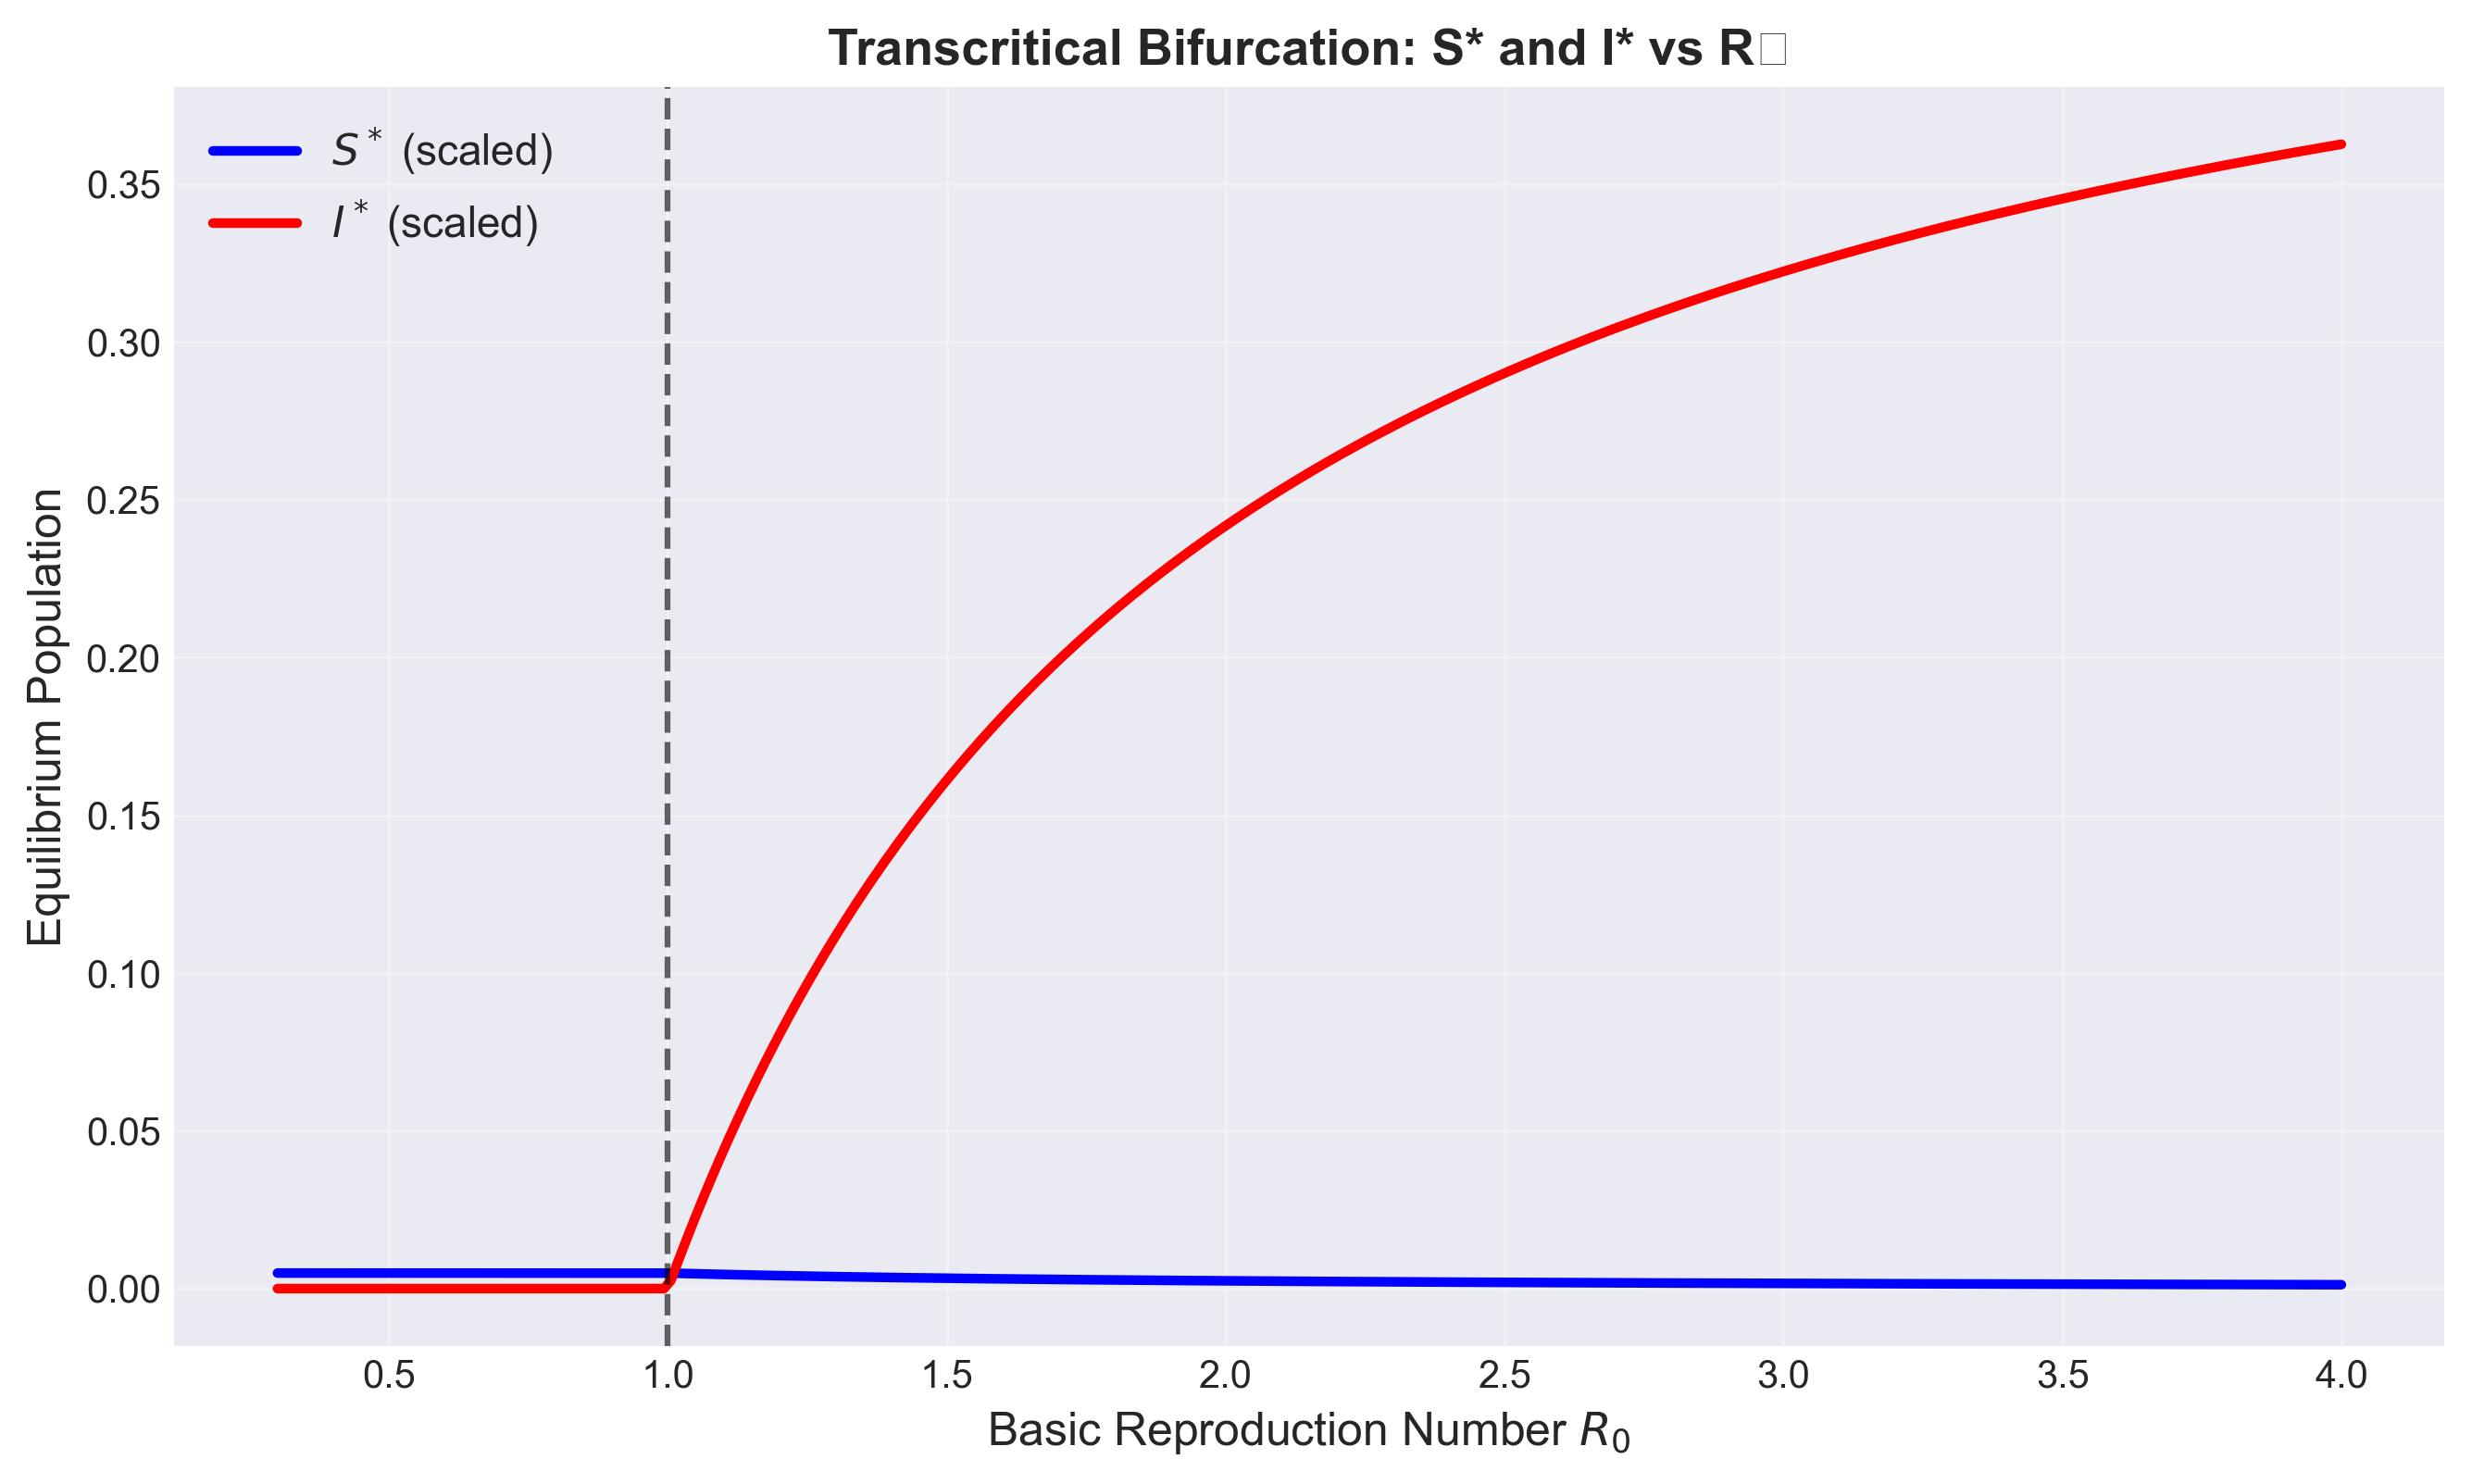
\includegraphics[width=0.85\textwidth]{BifurCordi.png}
    \caption{Transcritical bifurcation of the COVID-19 epidemiological model with respect to the basic reproduction number $R_0$. For $R_0 \leq 1$, the disease-free equilibrium is stable with a constant susceptible population and zero infected individuals. When $R_0 > 1$, an endemic equilibrium emerges, leading to a decrease in the susceptible population and an increase in the infected population. The intersection point $(S^* = I^*)$ indicates a population parity coordinate and confirms the occurrence of a transcritical bifurcation.}
    \label{fig:transcritical_bifurcation}
\end{figure}


\[
S^* = \frac{A}{d + pM}
\]
and zero infected individuals ($I^* = 0$). When $R_0 > 1$, the DFE loses stability and an endemic equilibrium emerges, where the susceptible population decreases according to
\[
S^* = \frac{S_{\text{DFE}}}{R_0},
\]
while the infected population $I^*$ increases as a function of $R_0$. The infected equilibrium is computed by first determining the exposed class at equilibrium,
\[
E^* = \frac{A - (d + pM)S^*}{b_2 + \alpha + \sigma + d},
\]
and then relating it to the infected class using the equilibrium ratio
\[
I^* = E^* \left( \frac{\alpha + \dfrac{c b_2}{b_1 + c + d}}{\eta + d + \delta} \right),
\]
which follows from the steady-state balance of the quarantine and infection compartments. The intersection point where $S^* = I^*$ is obtained analytically by equating the equilibrium expressions, yielding a population parity coordinate at $R_0 \approx 3.72$. This intersection highlights the qualitative exchange of stability between equilibria, confirming the presence of a transcritical bifurcation and emphasizing the critical role of $R_0$ in governing disease persistence.

\section{$R_0$ vs Model Parameters}

The variation of the basic reproduction number $R_0$ with respect to the transmission rate $\beta$ is illustrated in Figure~\ref{fig:R0_beta}. The relationship between $R_0$ and $\beta$ is linear, as $\beta$ appears in the numerator of the expression
\[
R_0 = \frac{A \beta (1-\rho_1)(1-\rho_2)}{(d + pM)(b_2 + \alpha + \sigma + d)}.
\]
An increase in the transmission rate directly amplifies disease spread, leading to higher values of $R_0$. The marked intersection point at $\beta \approx 1.40$ corresponds to the critical transmission threshold where $R_0 = 1$. For $\beta < 1.40$, the disease-free equilibrium remains stable, whereas for $\beta > 1.40$, the system transitions to an endemic state, indicating sustained disease transmission.

\begin{figure}[H]
    \centering
    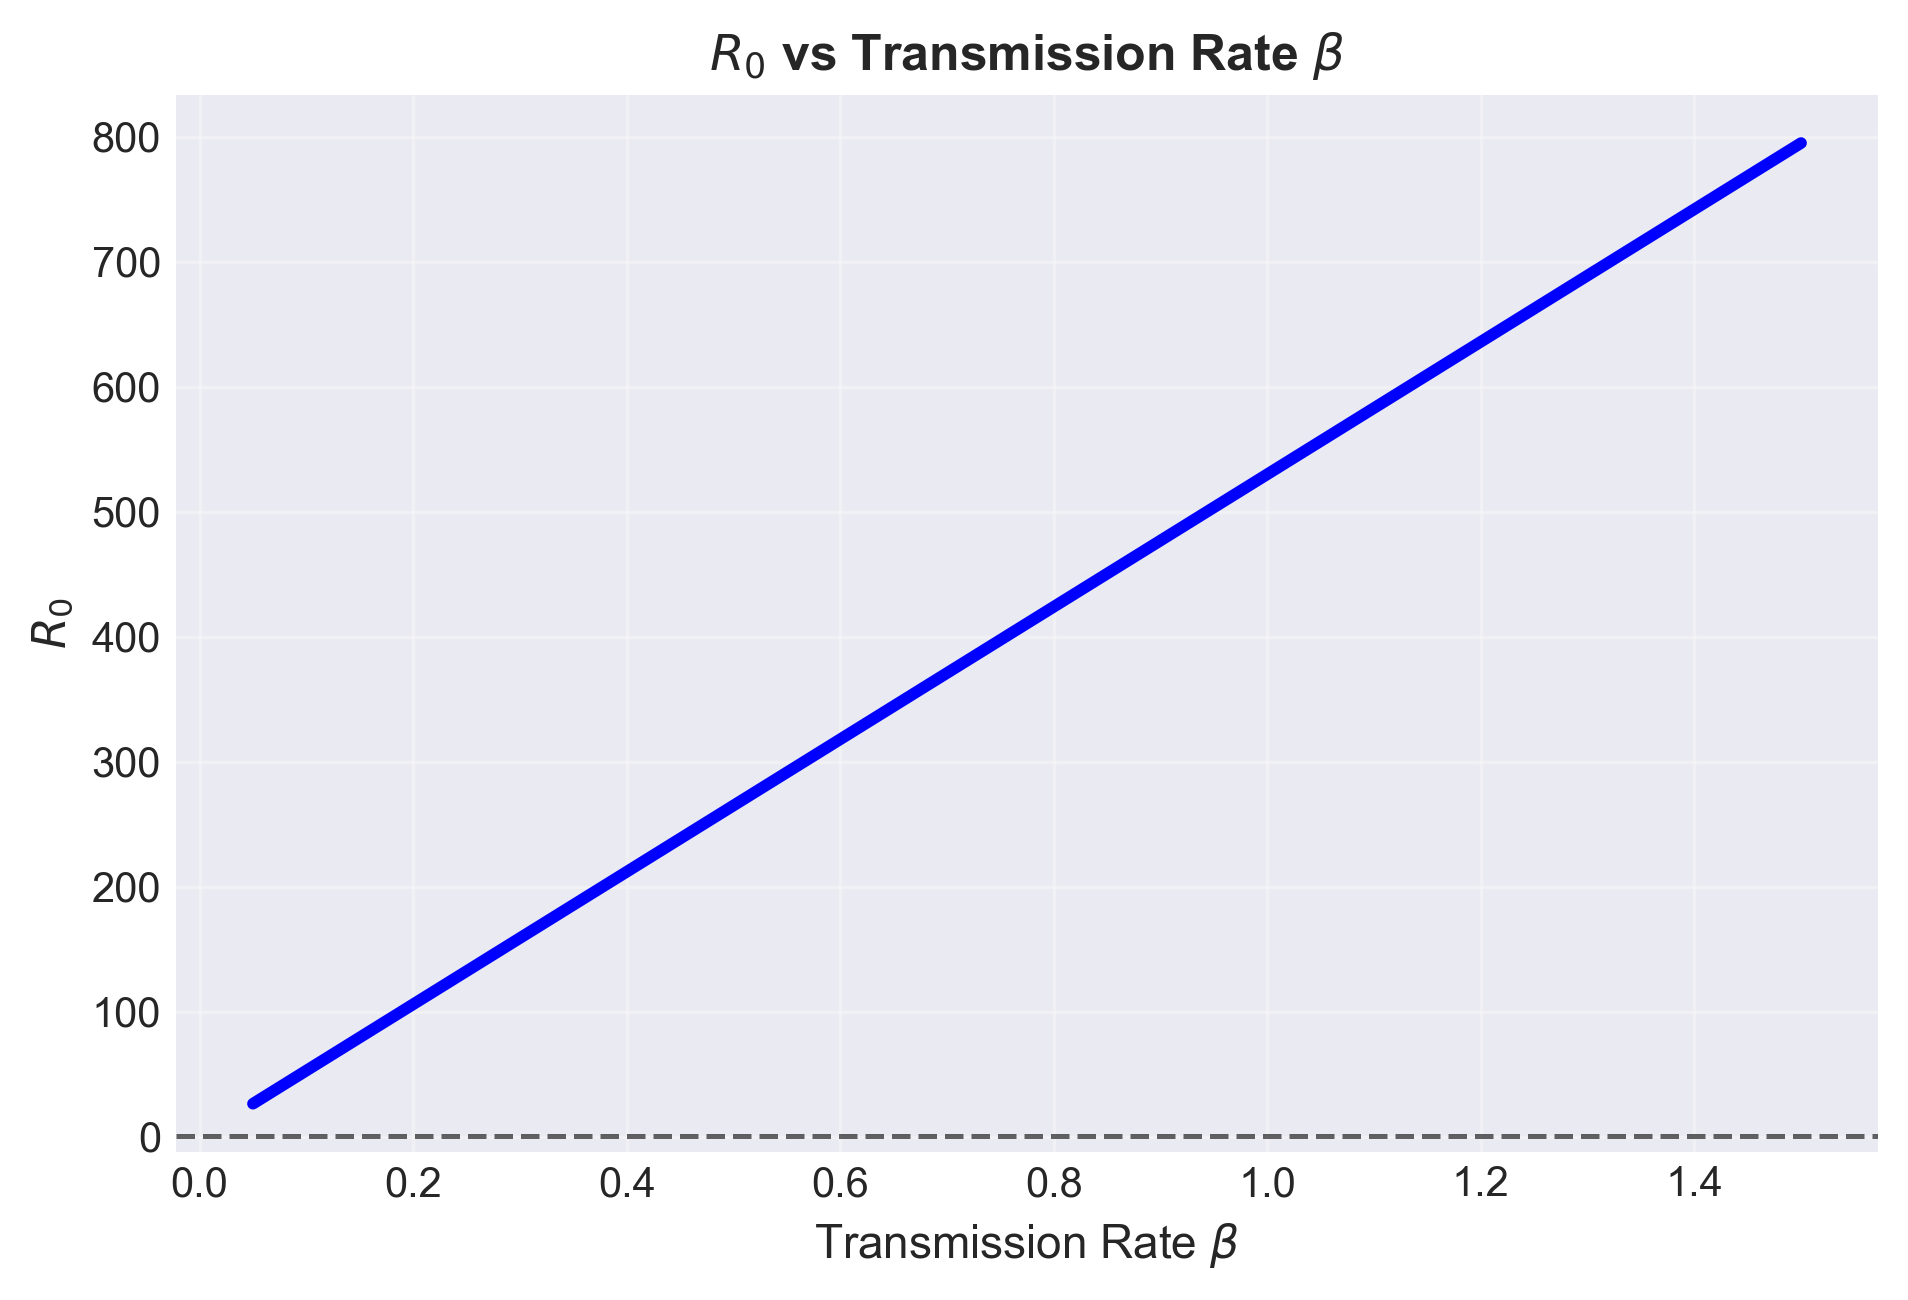
\includegraphics[width=0.55\linewidth]{R_beta_coord.png}
    \caption{$R_0$ as a function of the transmission rate $\beta$, showing the critical threshold at $R_0 = 1$.}
    \label{fig:R0_beta}
\end{figure}

The impact of the disease onset rate $\alpha$ on the basic reproduction number is shown in Figure~\ref{fig:R0_alpha}. As $\alpha$ appears in the denominator of the $R_0$ expression, increasing $\alpha$ reduces the average time individuals spend in the exposed class, thereby decreasing secondary infections. The curve exhibits a nonlinear decreasing trend, with a critical onset rate at $\alpha \approx 2.54$ where $R_0 = 1$. This threshold signifies the transition from endemic persistence ($R_0 > 1$) to disease elimination ($R_0 < 1$), highlighting the importance of rapid disease detection and isolation.

\begin{figure}[H]
    \centering
    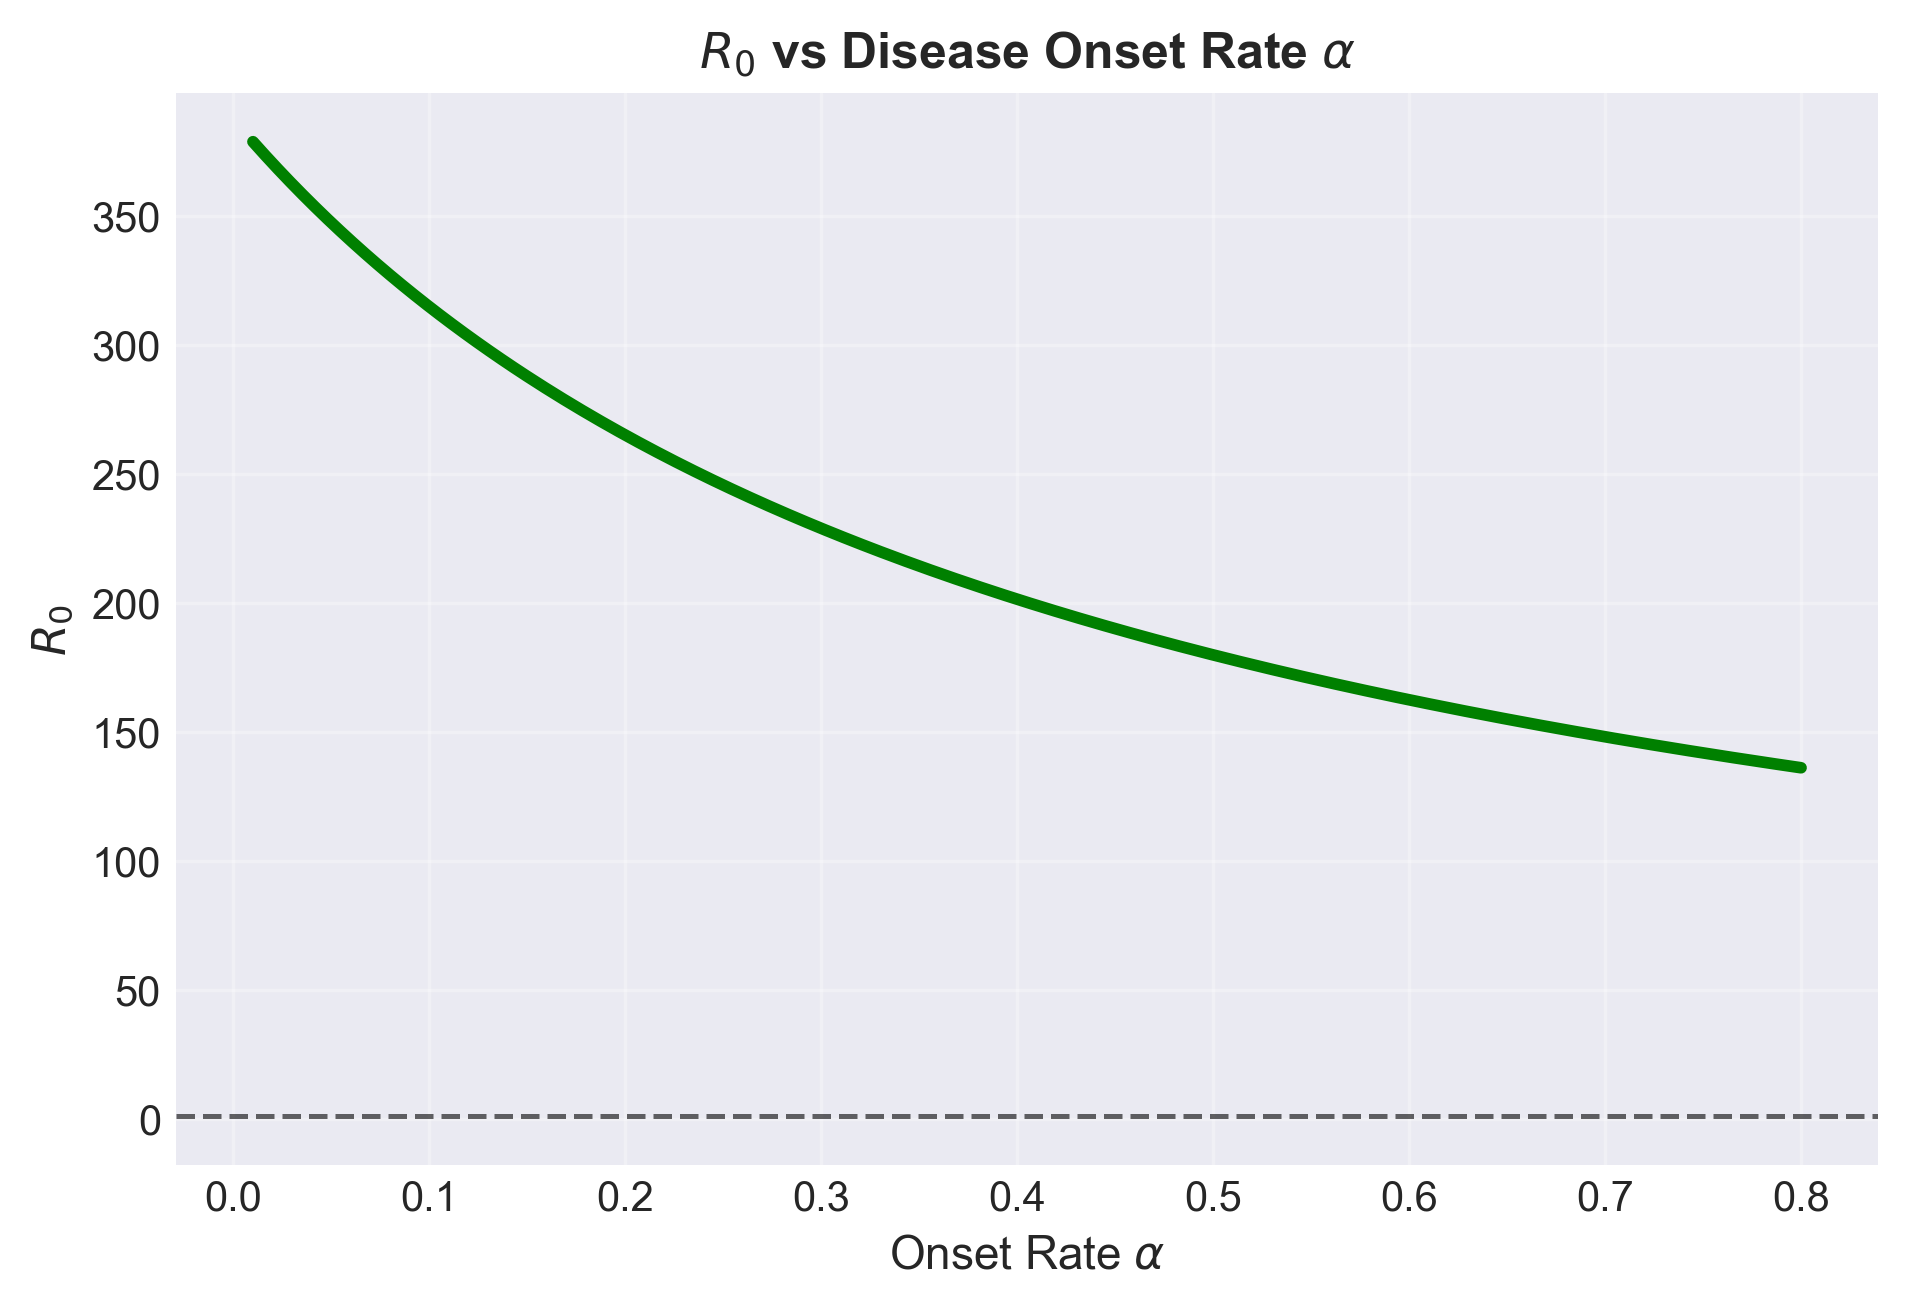
\includegraphics[width=0.55\linewidth]{R_vs_alpha.png}
    \caption{$R_0$ variation with respect to the onset rate $\alpha$, illustrating the stabilizing effect of faster disease progression to isolation.}
    \label{fig:R0_alpha}
\end{figure}

Figure~\ref{fig:R0_b2} illustrates the dependence of the basic reproduction number on the quarantine rate $b_2$. An increase in $b_2$ enhances the movement of exposed individuals into quarantine, effectively reducing their contribution to disease transmission. Consequently, $R_0$ decreases nonlinearly as $b_2$ increases. The critical quarantine rate is observed at $b_2 \approx 3.04$, where $R_0$ crosses the unity threshold. This result underscores the crucial role of effective quarantine strategies in suppressing epidemic outbreaks.

\begin{figure}[H]
    \centering
    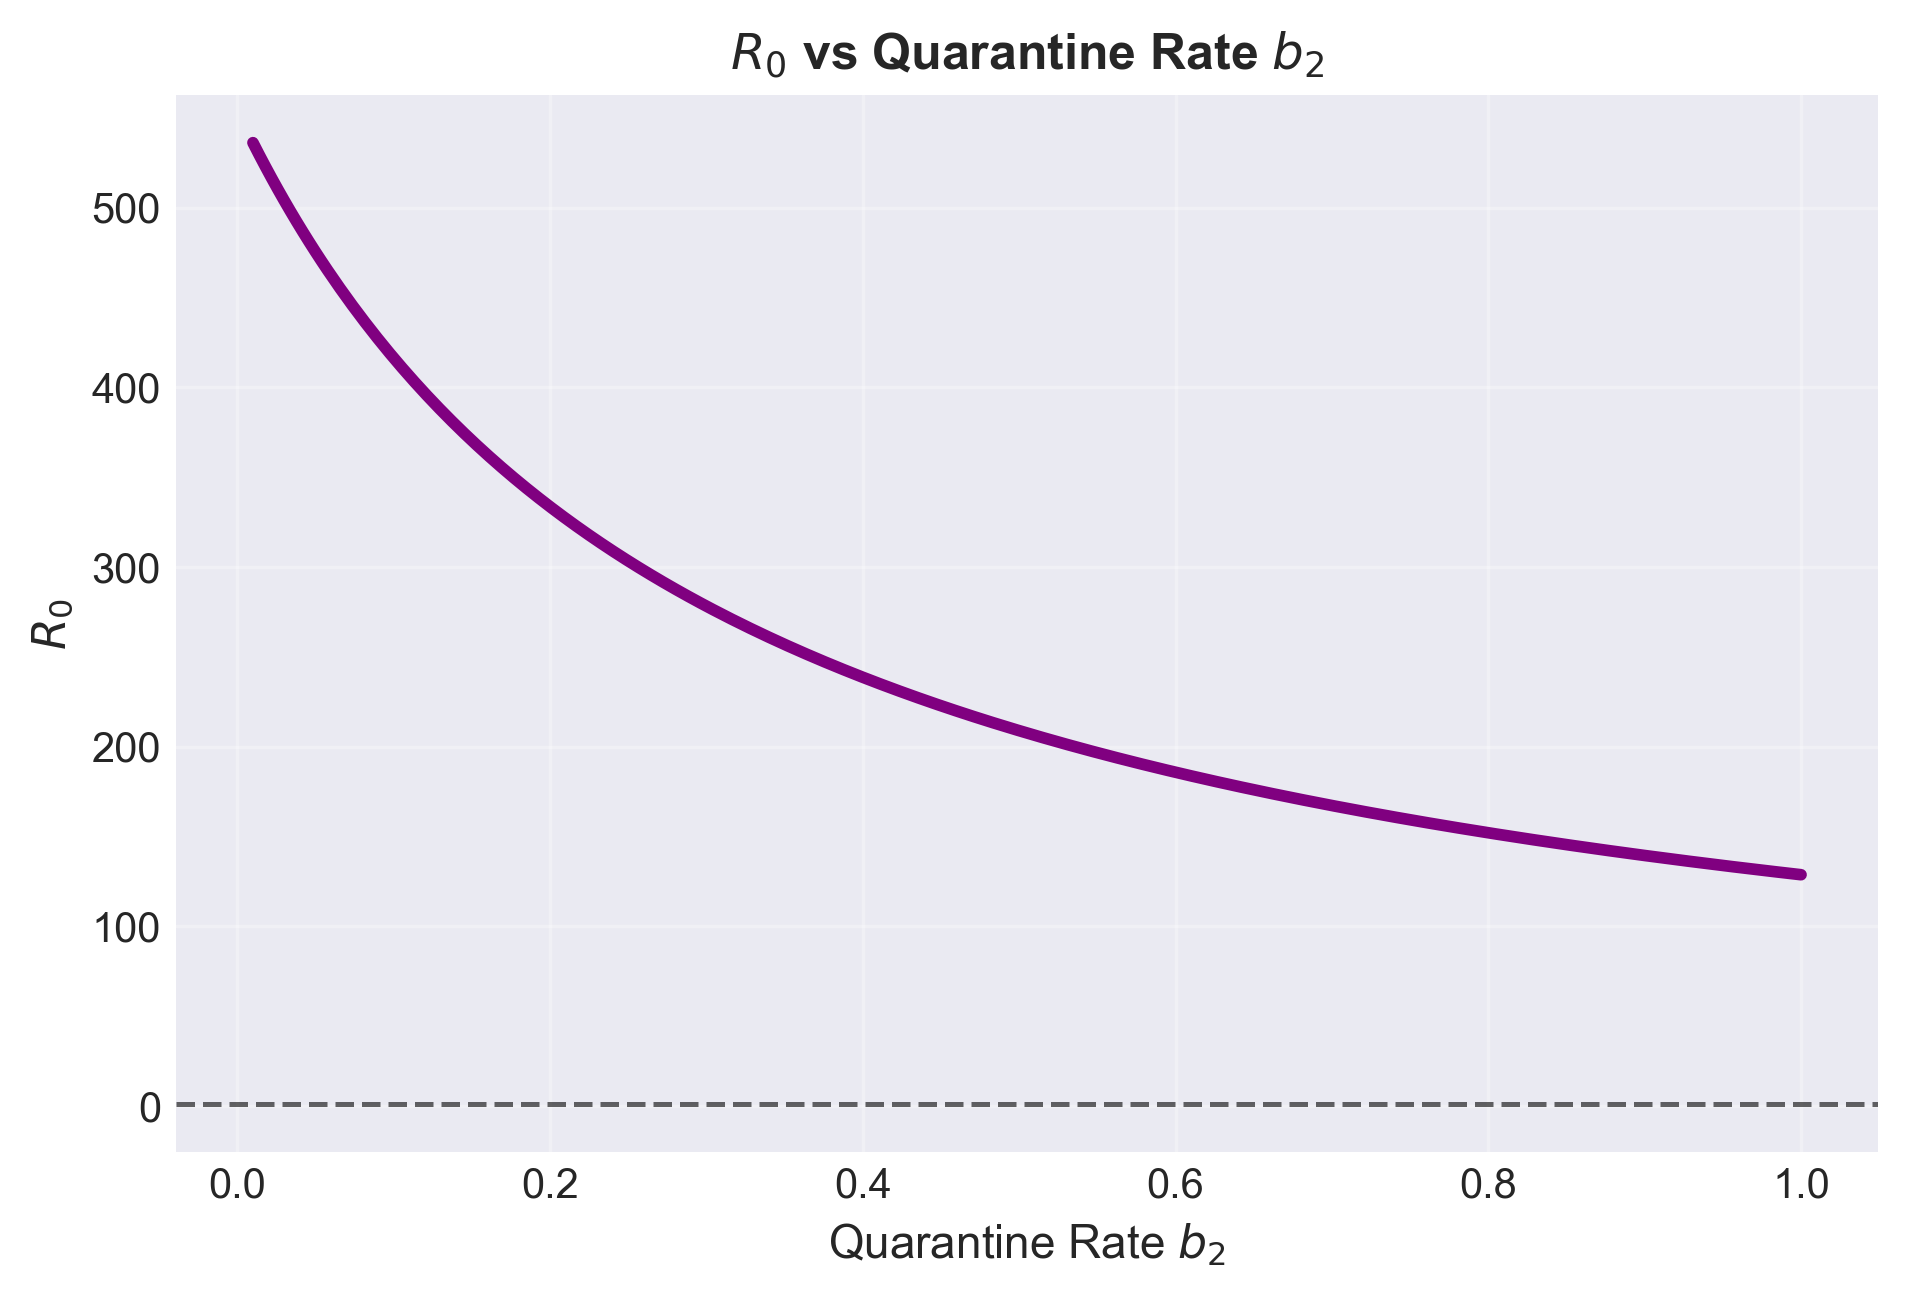
\includegraphics[width=0.55\linewidth]{R_vs_b2Coord.png}
    \caption{$R_0$ as a function of the quarantine rate $b_2$, showing the threshold required for disease control.}
    \label{fig:R0_b2}
\end{figure}

The effect of the protection rate $\rho_2$ on the basic reproduction number is depicted in Figure~\ref{fig:R0_rho2}. Since $\rho_2$ represents the fraction of the population adopting protective measures, it directly reduces effective contact rates through the term $(1-\rho_2)$. As a result, $R_0$ decreases sharply with increasing $\rho_2$, demonstrating a strong monotonic decline. The critical protection level is identified at $\rho_2 \approx 0.97$, where $R_0 = 1$. This emphasizes the effectiveness of large-scale preventive measures such as social distancing, mask usage, and public awareness in controlling disease spread.

\begin{figure}[H]
    \centering
    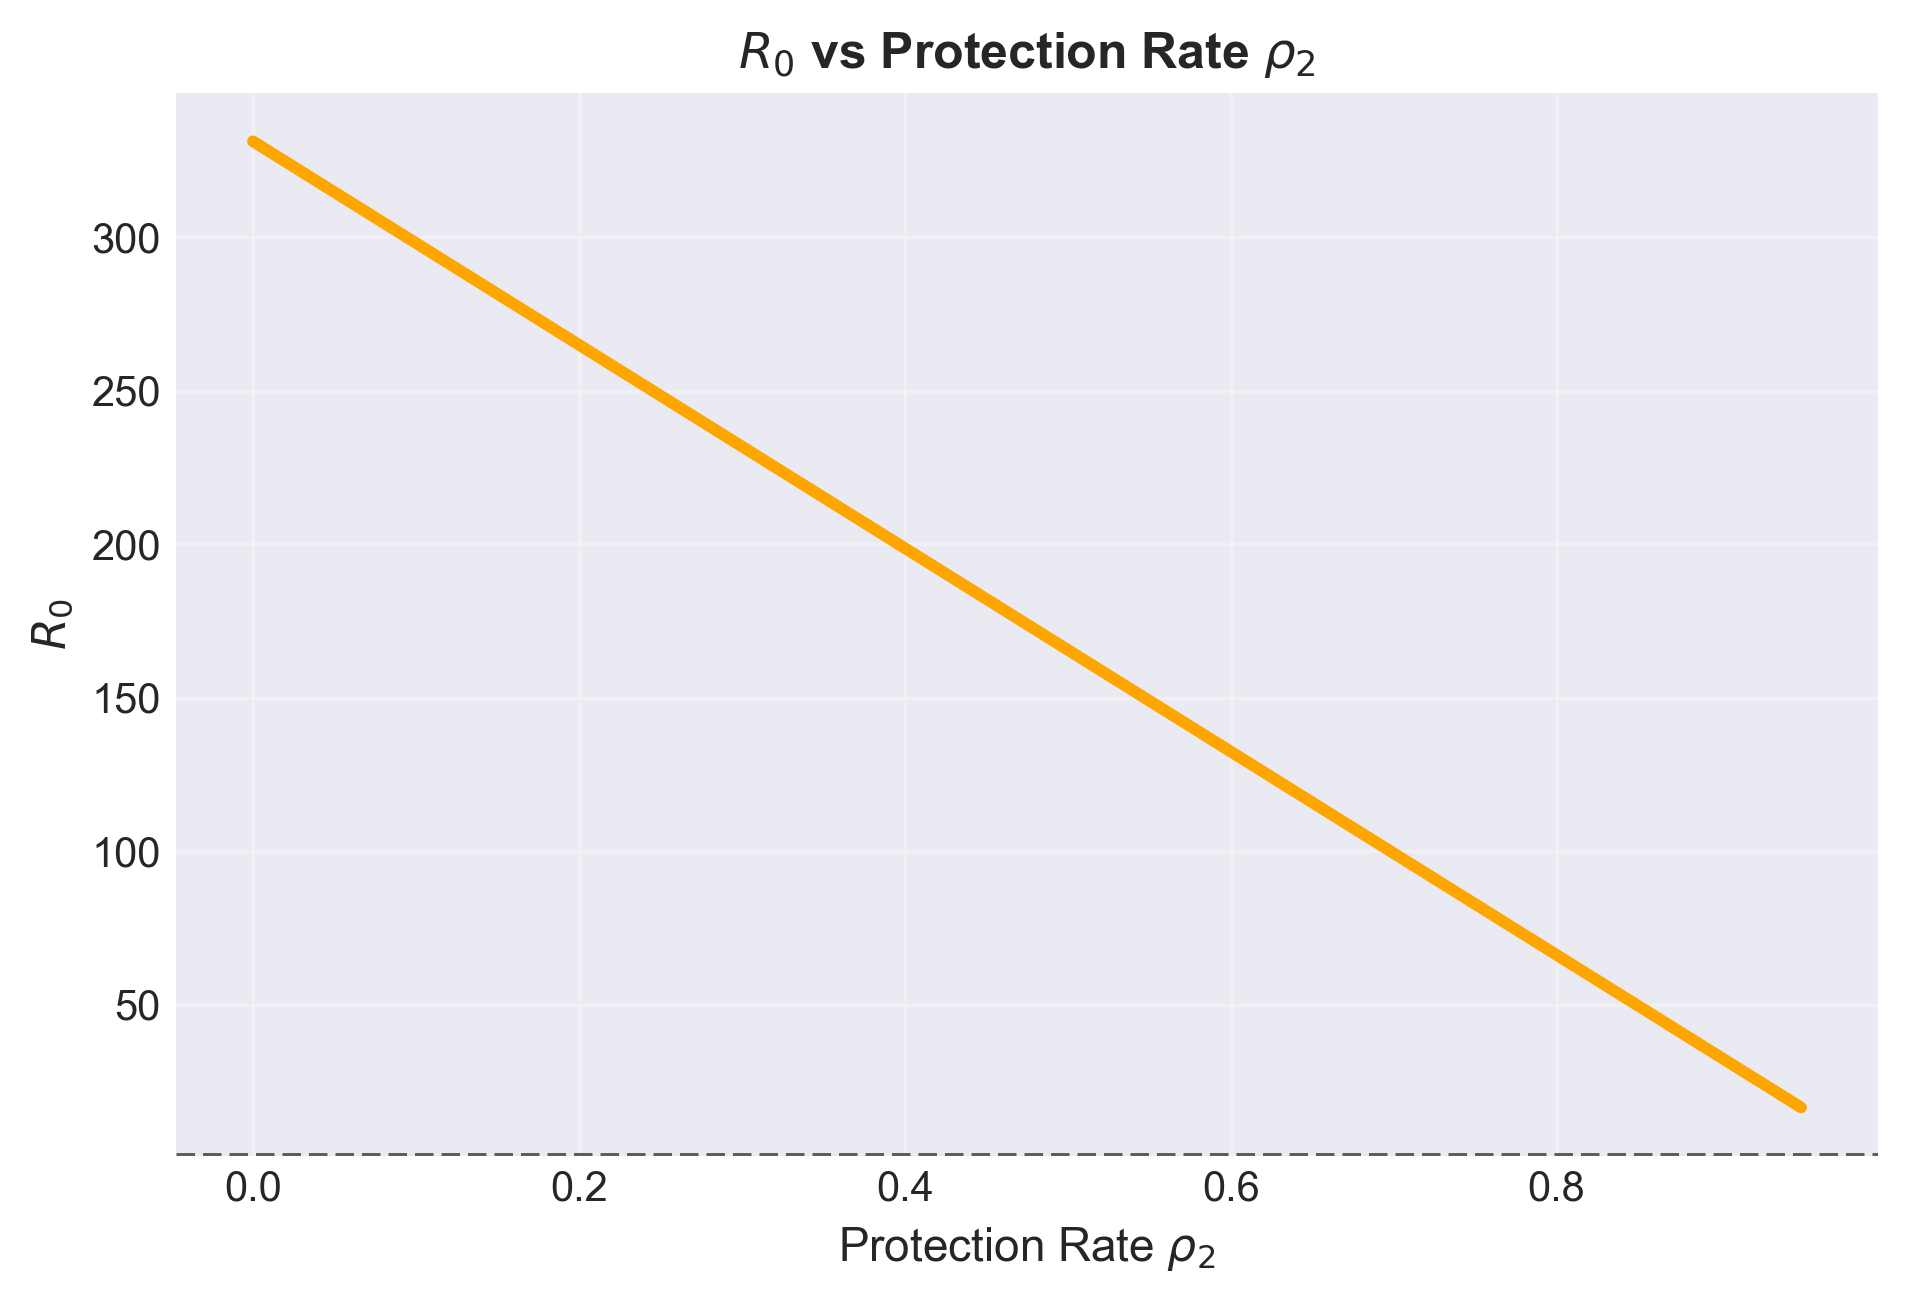
\includegraphics[width=0.55\linewidth]{R_vs_rho2Coord.png}
    \caption{$R_0$ variation with respect to the protection rate $\rho_2$, highlighting the importance of preventive interventions.}
    \label{fig:R0_rho2}
\end{figure}

\section{Two-Parameter Bifurcation Analysis}

This section presents a two-parameter bifurcation analysis of the COVID-19 epidemiological model to examine the combined influence of key parameters on the basic reproduction number $R_0$. The bifurcation diagrams are generated by evaluating the threshold condition $R_0 = 1$, which separates the disease-free equilibrium (DFE) from the endemic equilibrium (EE). Regions corresponding to $R_0 < 1$ indicate disease elimination, while regions with $R_0 > 1$ represent sustained disease transmission.

The bifurcation diagram in Figure~\ref{fig:alpha_beta} illustrates the joint effect of the disease onset rate $\alpha$ and the transmission rate $\beta$ on $R_0$. Higher transmission rates increase $R_0$, whereas larger values of $\alpha$ reduce the time individuals spend in the exposed class, thereby lowering disease transmission. The red threshold curve represents the critical boundary where $R_0 = 1$, separating the disease-free equilibrium region (DFE) from the endemic equilibrium region (EE). This plot highlights the trade-off between transmission intensity and early disease progression.

\begin{figure}[H]
    \centering
    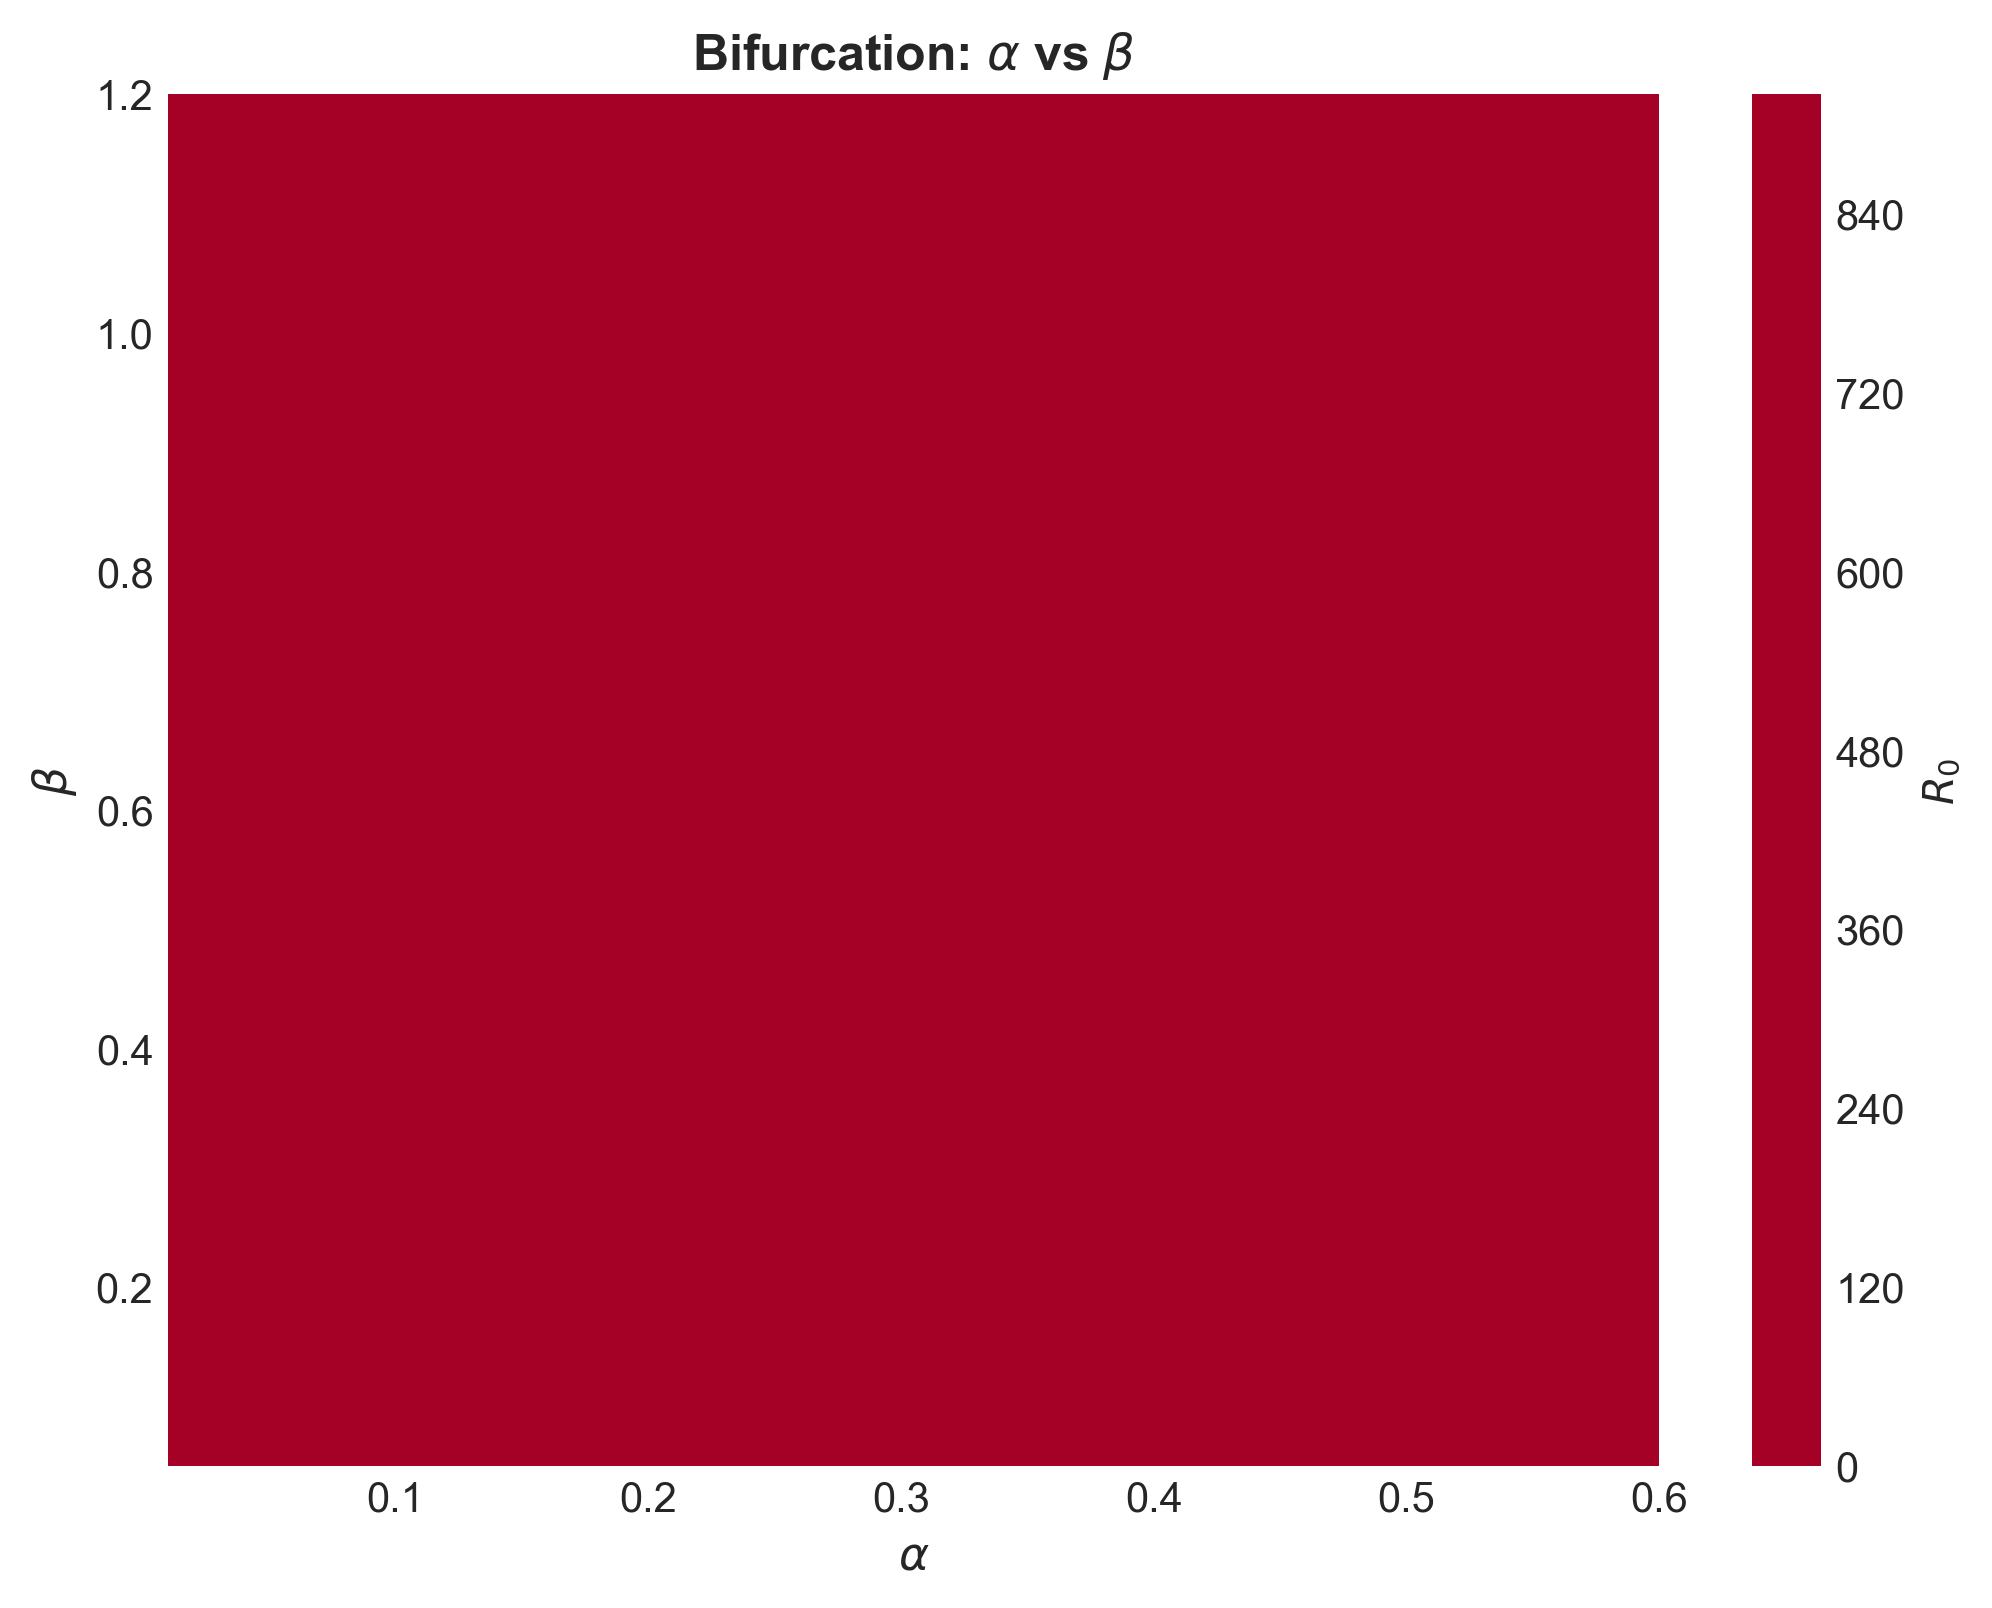
\includegraphics[width=0.55\linewidth]{alpha_vs_beta_onR.png}
    \caption{Two-parameter bifurcation diagram in the $(\alpha, \beta)$ plane showing regions of disease-free equilibrium (DFE) and endemic equilibrium (EE).}
    \label{fig:alpha_beta}
\end{figure}

Figure~\ref{fig:rho1_rho2} depicts the combined impact of the government intervention rate $\rho_1$ and the protection rate $\rho_2$ on disease dynamics. Both parameters reduce effective contact rates, and increasing either parameter shifts the system toward the disease-free equilibrium. The bifurcation curve demonstrates that strong preventive measures can compensate for weaker governmental intervention, emphasizing the importance of public compliance and awareness in controlling COVID-19 spread.

\begin{figure}[H]
    \centering
    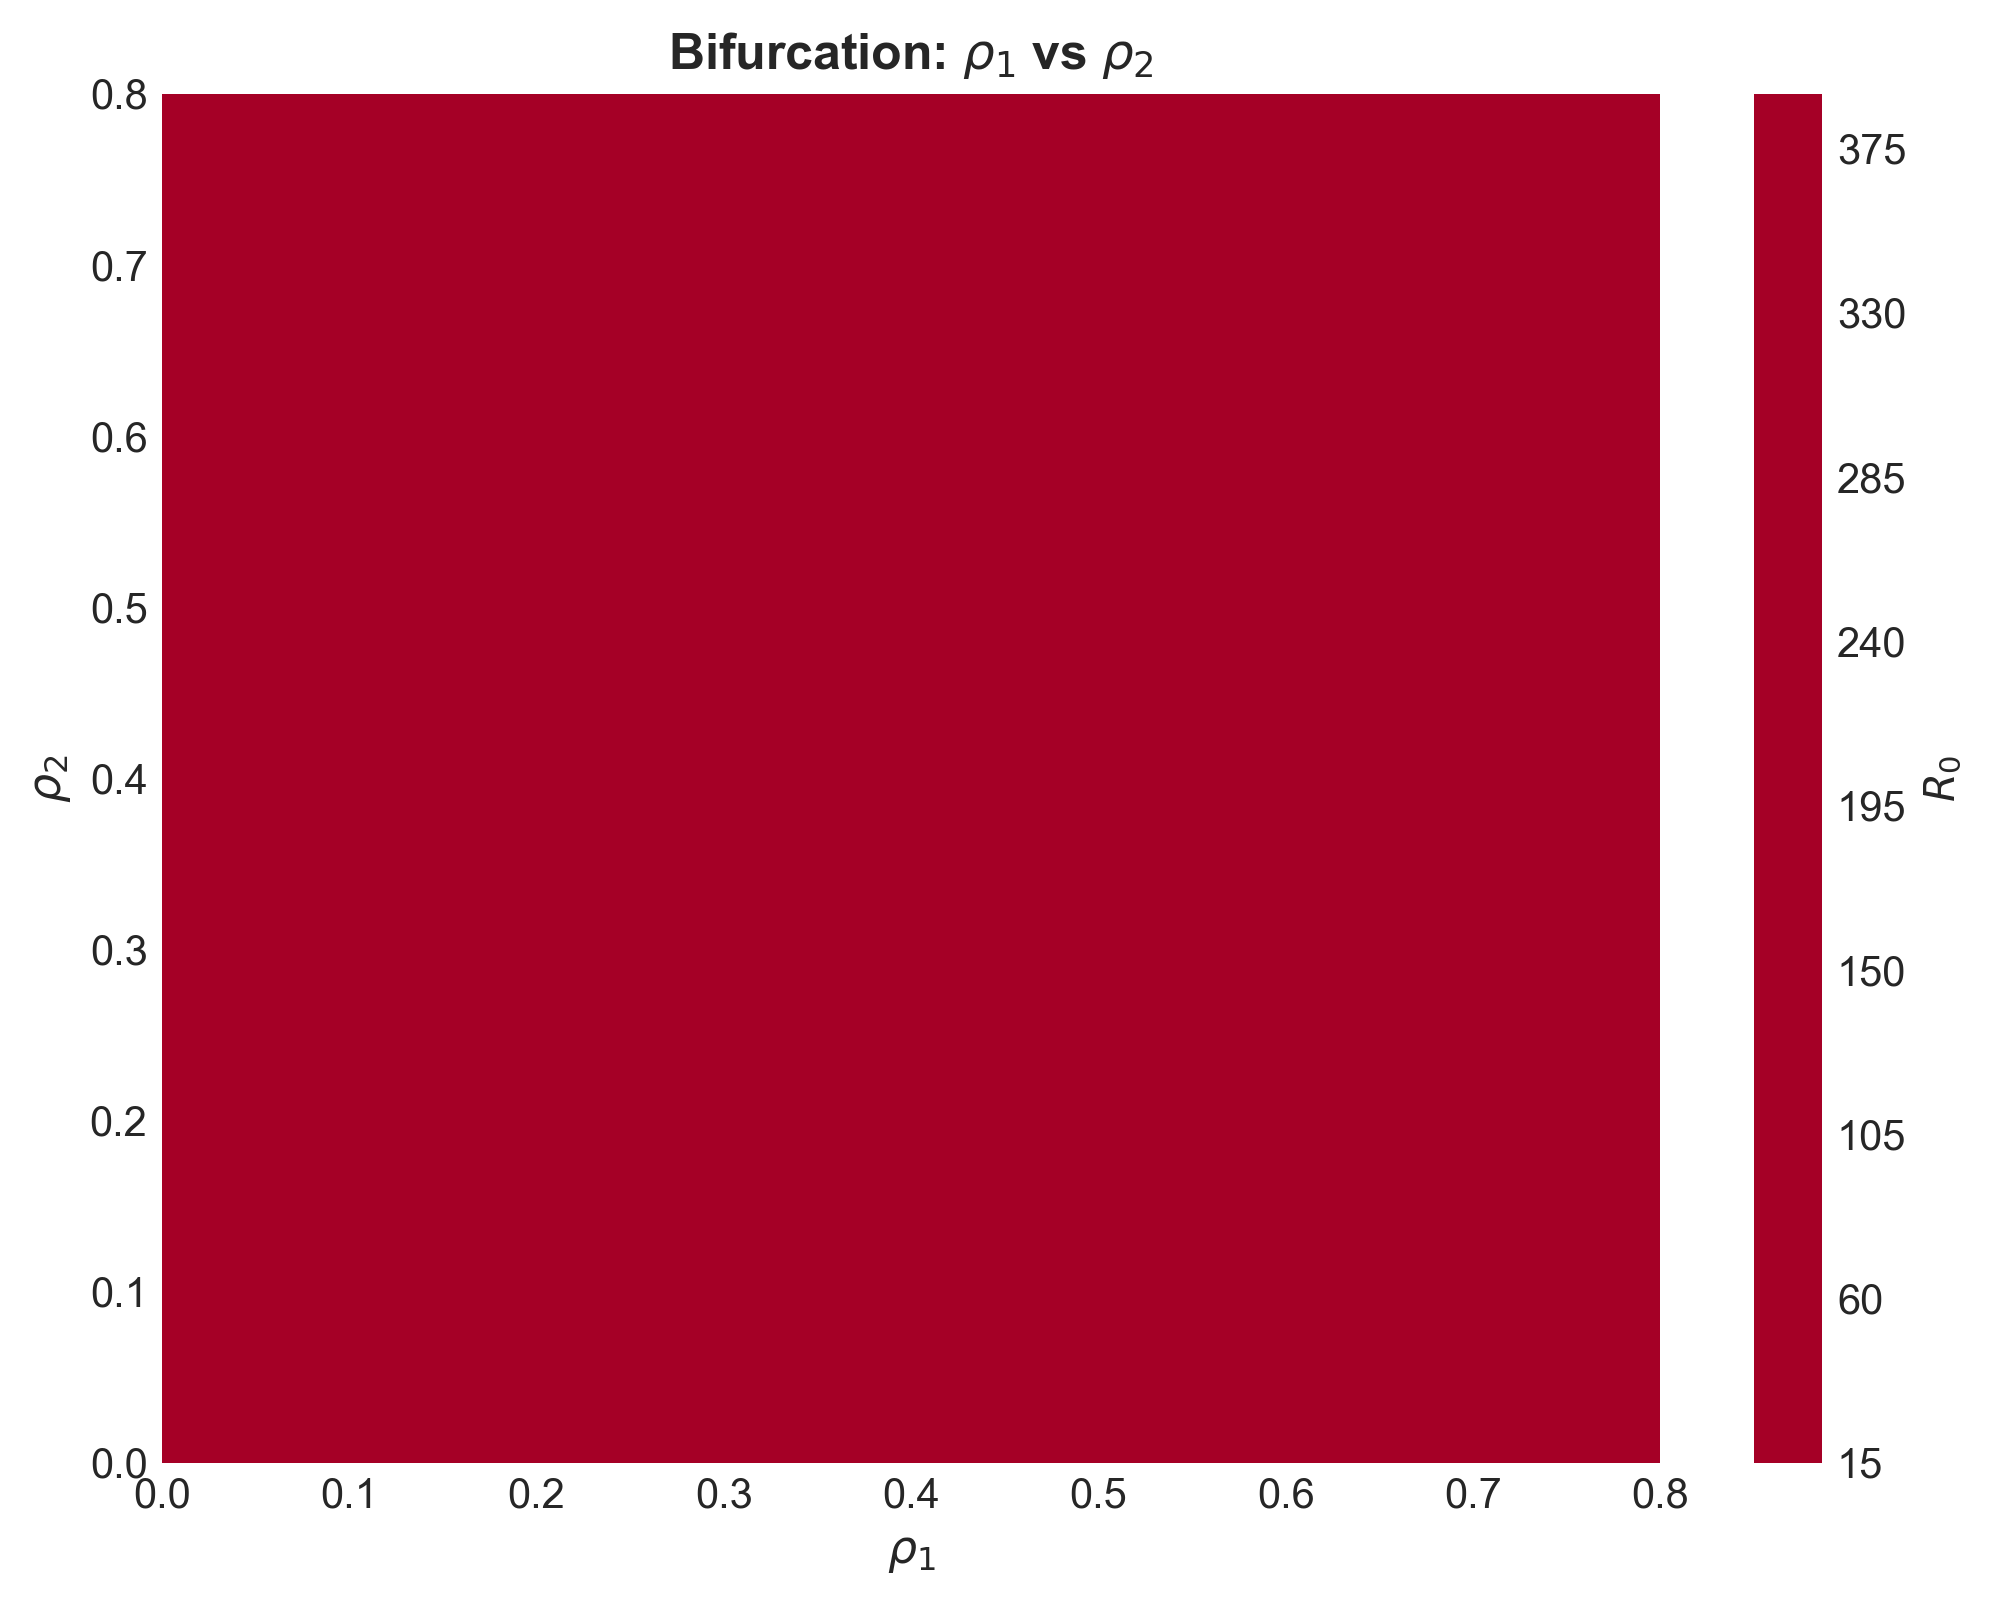
\includegraphics[width=0.55\linewidth]{rho1_vs_rho2onR.png}
    \caption{Two-parameter bifurcation diagram in the $(\rho_1, \rho_2)$ plane illustrating the stabilizing effects of intervention and protection measures.}
    \label{fig:rho1_rho2}
\end{figure}

Figure~\ref{fig:A_beta} illustrates the combined effect of the recruitment rate $A$ and the transmission rate $\beta$ on the basic reproduction number. An increase in population inflow enhances susceptibility, while higher transmission rates accelerate infection spread. The bifurcation boundary indicates that high transmission intensity can induce endemic behavior even for moderate recruitment levels.

\begin{figure}[H]
    \centering
    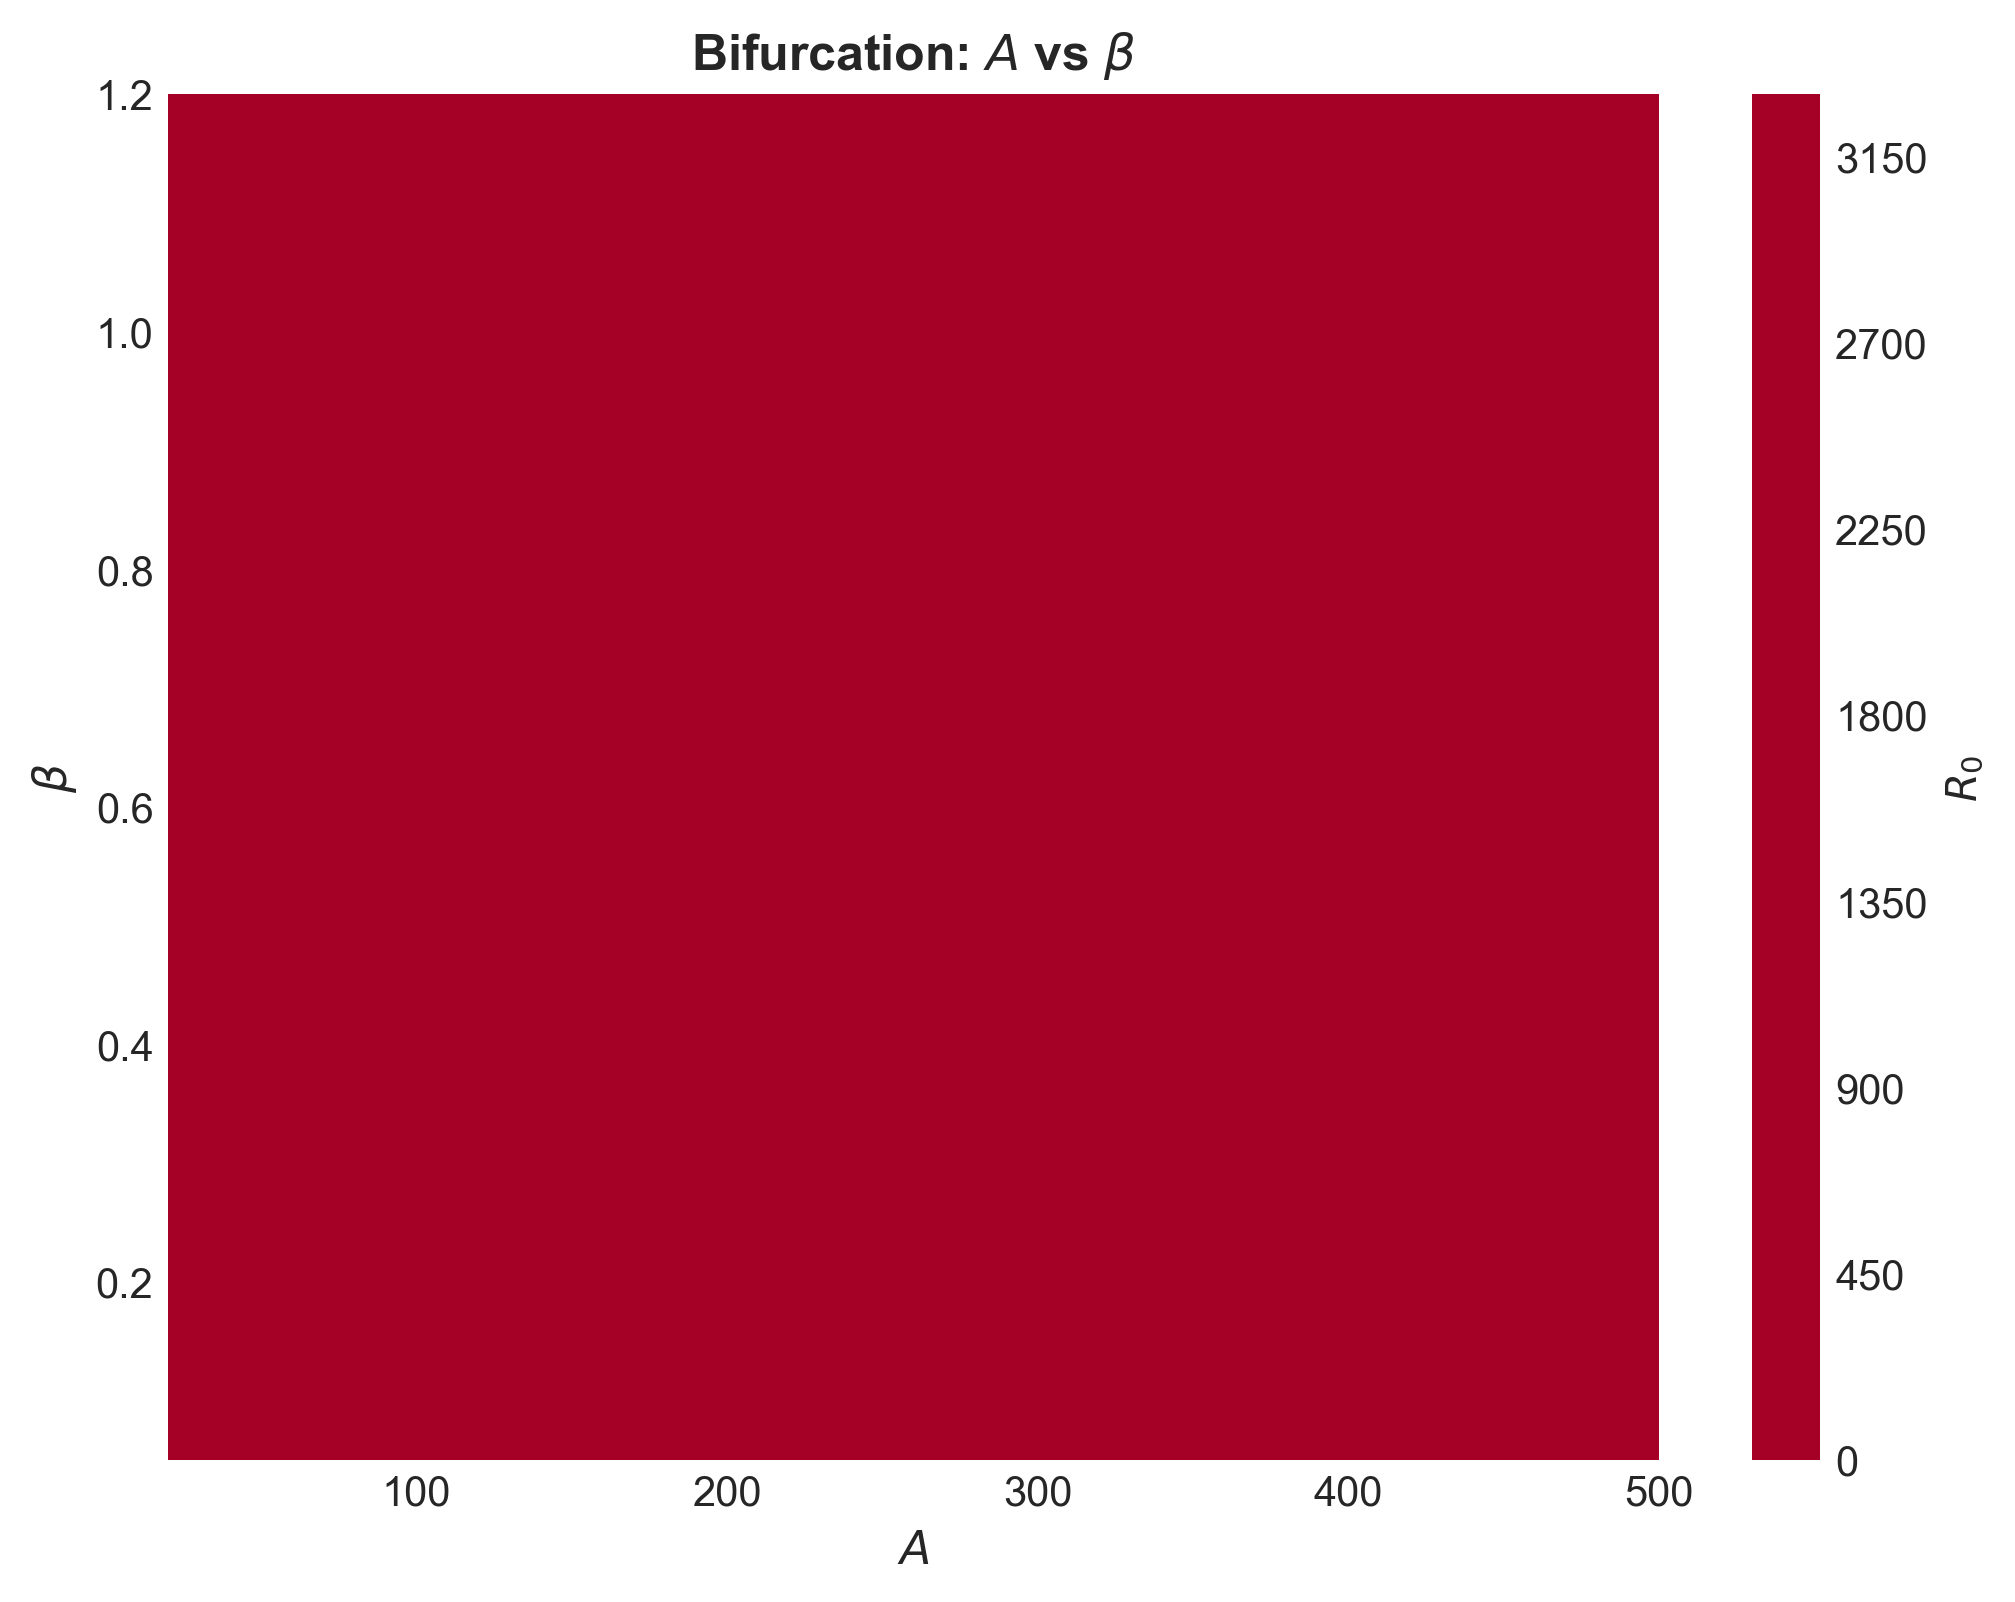
\includegraphics[width=0.55\linewidth]{A_vs_betaonR.png}
    \caption{Two-parameter bifurcation diagram in the $(A, \beta)$ plane highlighting the influence of population recruitment and transmission rate.}
    \label{fig:A_beta}
\end{figure}

Figure~\ref{fig:A_d} illustrates the combined effect of the recruitment rate $A$ and the natural death rate $d$ on disease dynamics. An increase in $A$ enlarges the susceptible population, promoting disease persistence, whereas higher values of $d$ reduce population size and infection potential. The bifurcation curve highlights that elevated natural mortality can counterbalance high recruitment, thereby stabilizing the disease-free equilibrium.

\begin{figure}[H]
    \centering
    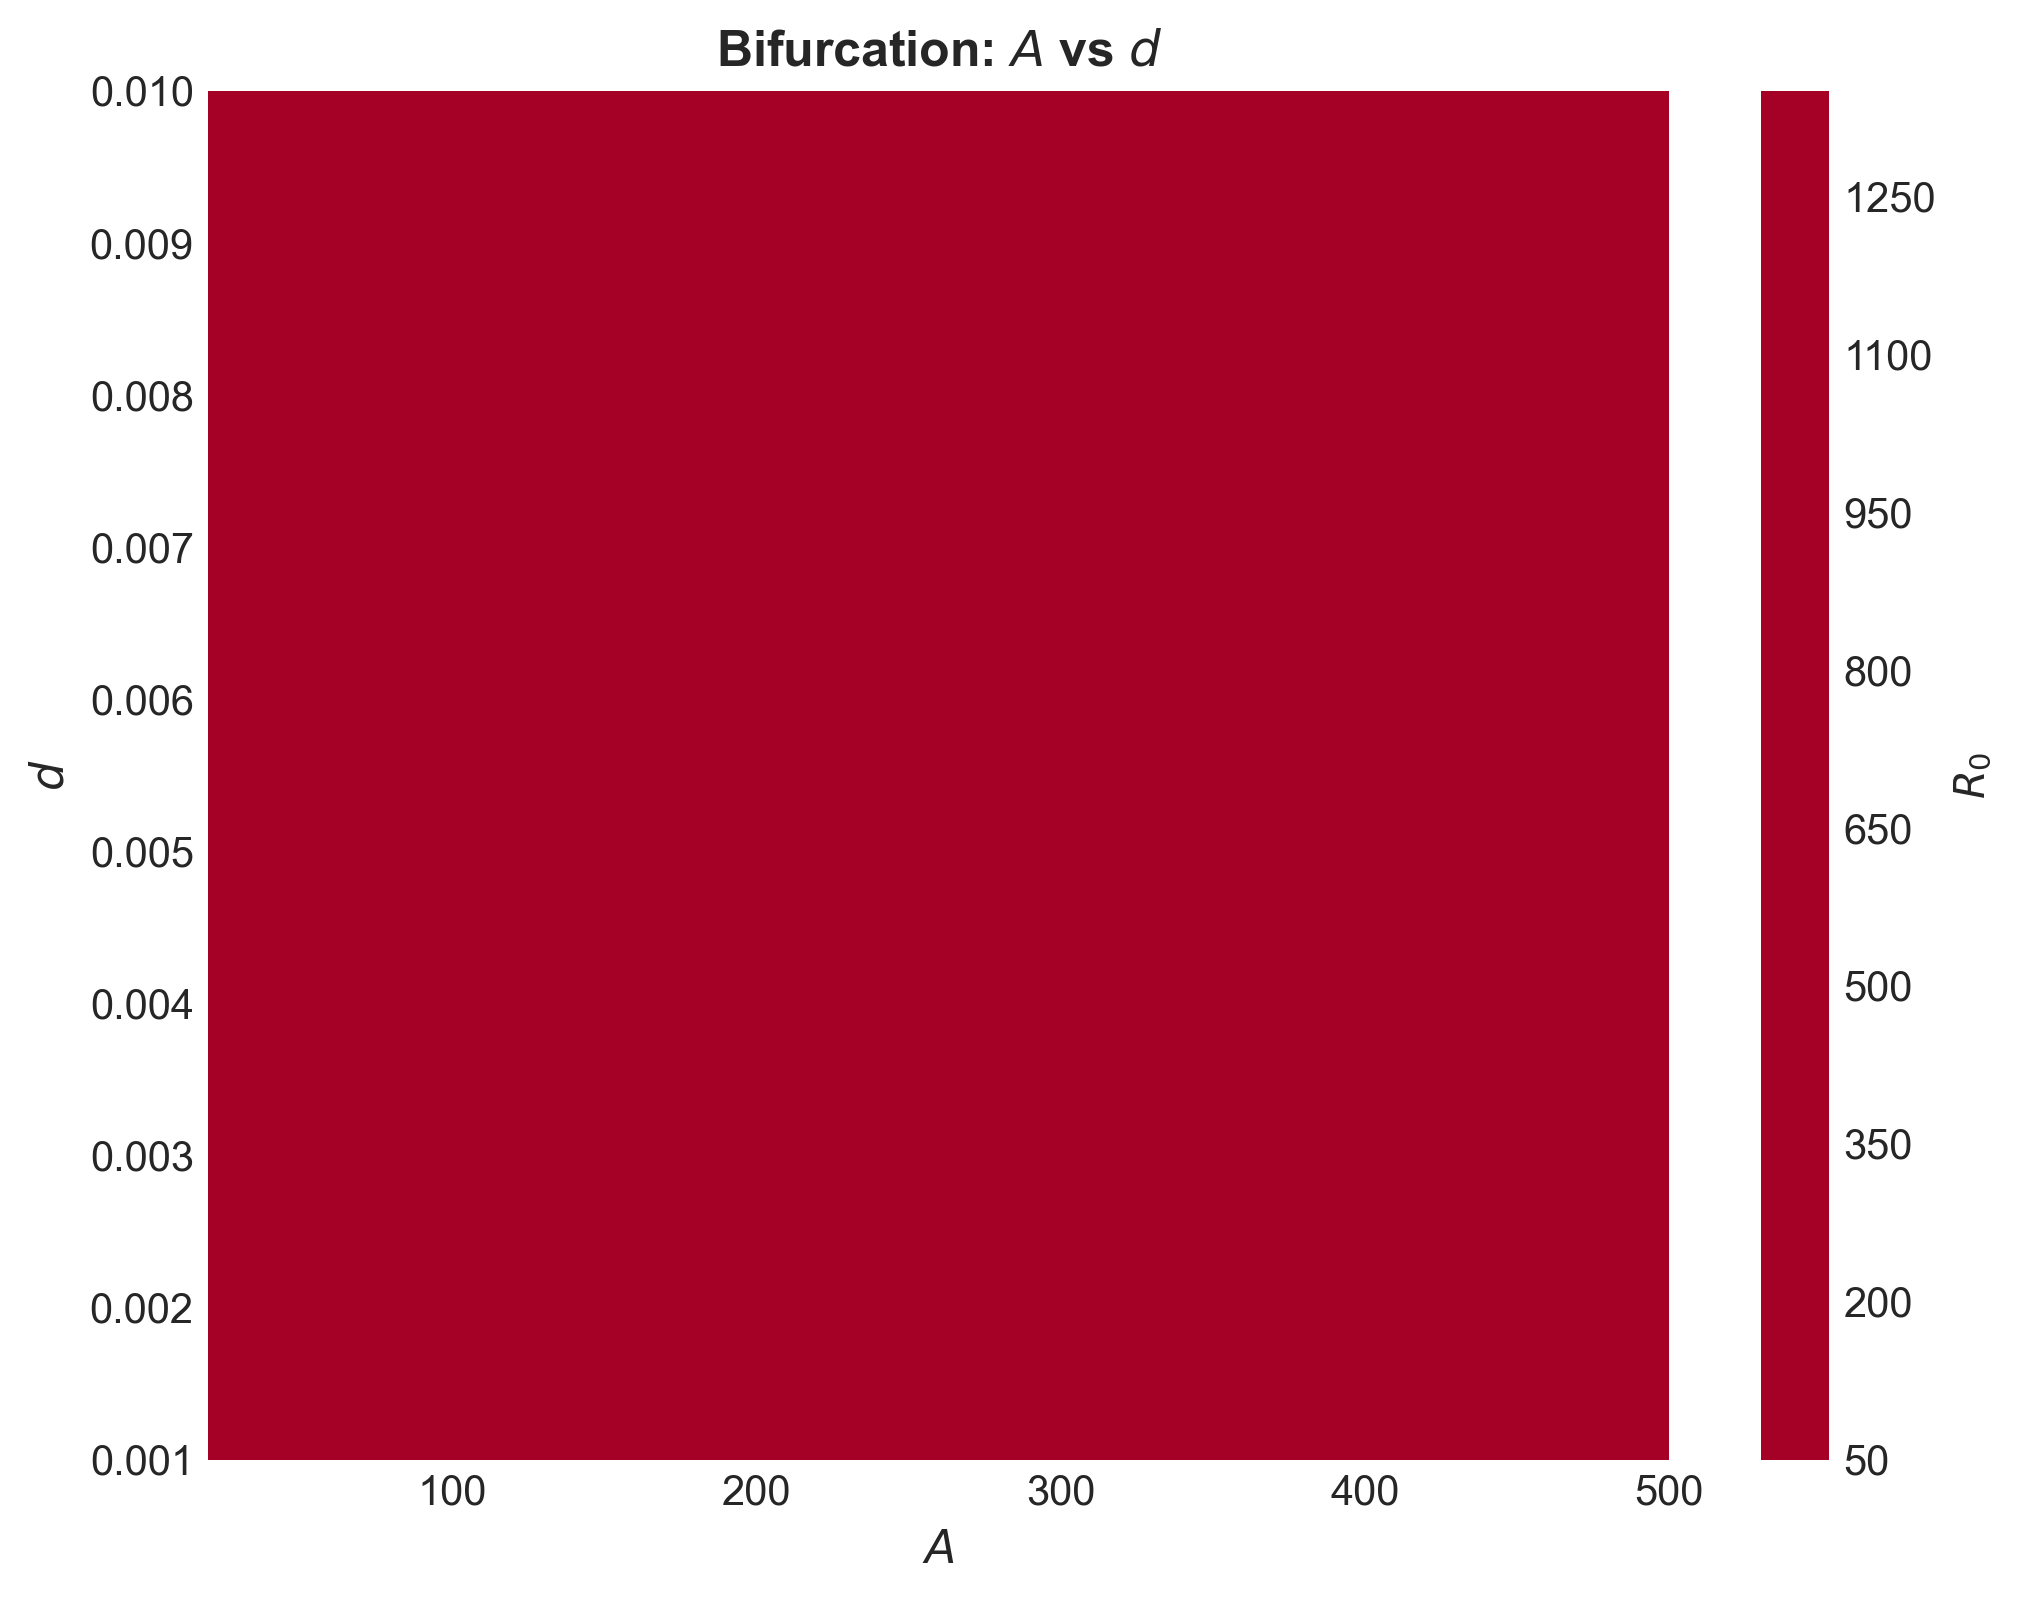
\includegraphics[width=0.55\linewidth]{A_vs_donR.png}
    \caption{Two-parameter bifurcation diagram in the $(A,d)$ plane showing DFE and EE regions separated by the threshold $R_0=1$.}
    \label{fig:A_d}
\end{figure}

Figure~\ref{fig:A_rho2} depicts the interaction between the recruitment rate $A$ and the precautionary measures parameter $\rho_2$. Increasing $\rho_2$ reduces effective contact rates and suppresses disease transmission, even under high recruitment conditions. The bifurcation boundary demonstrates that strong preventive measures can successfully maintain the disease-free equilibrium despite continuous population inflow.

\begin{figure}[H]
    \centering
    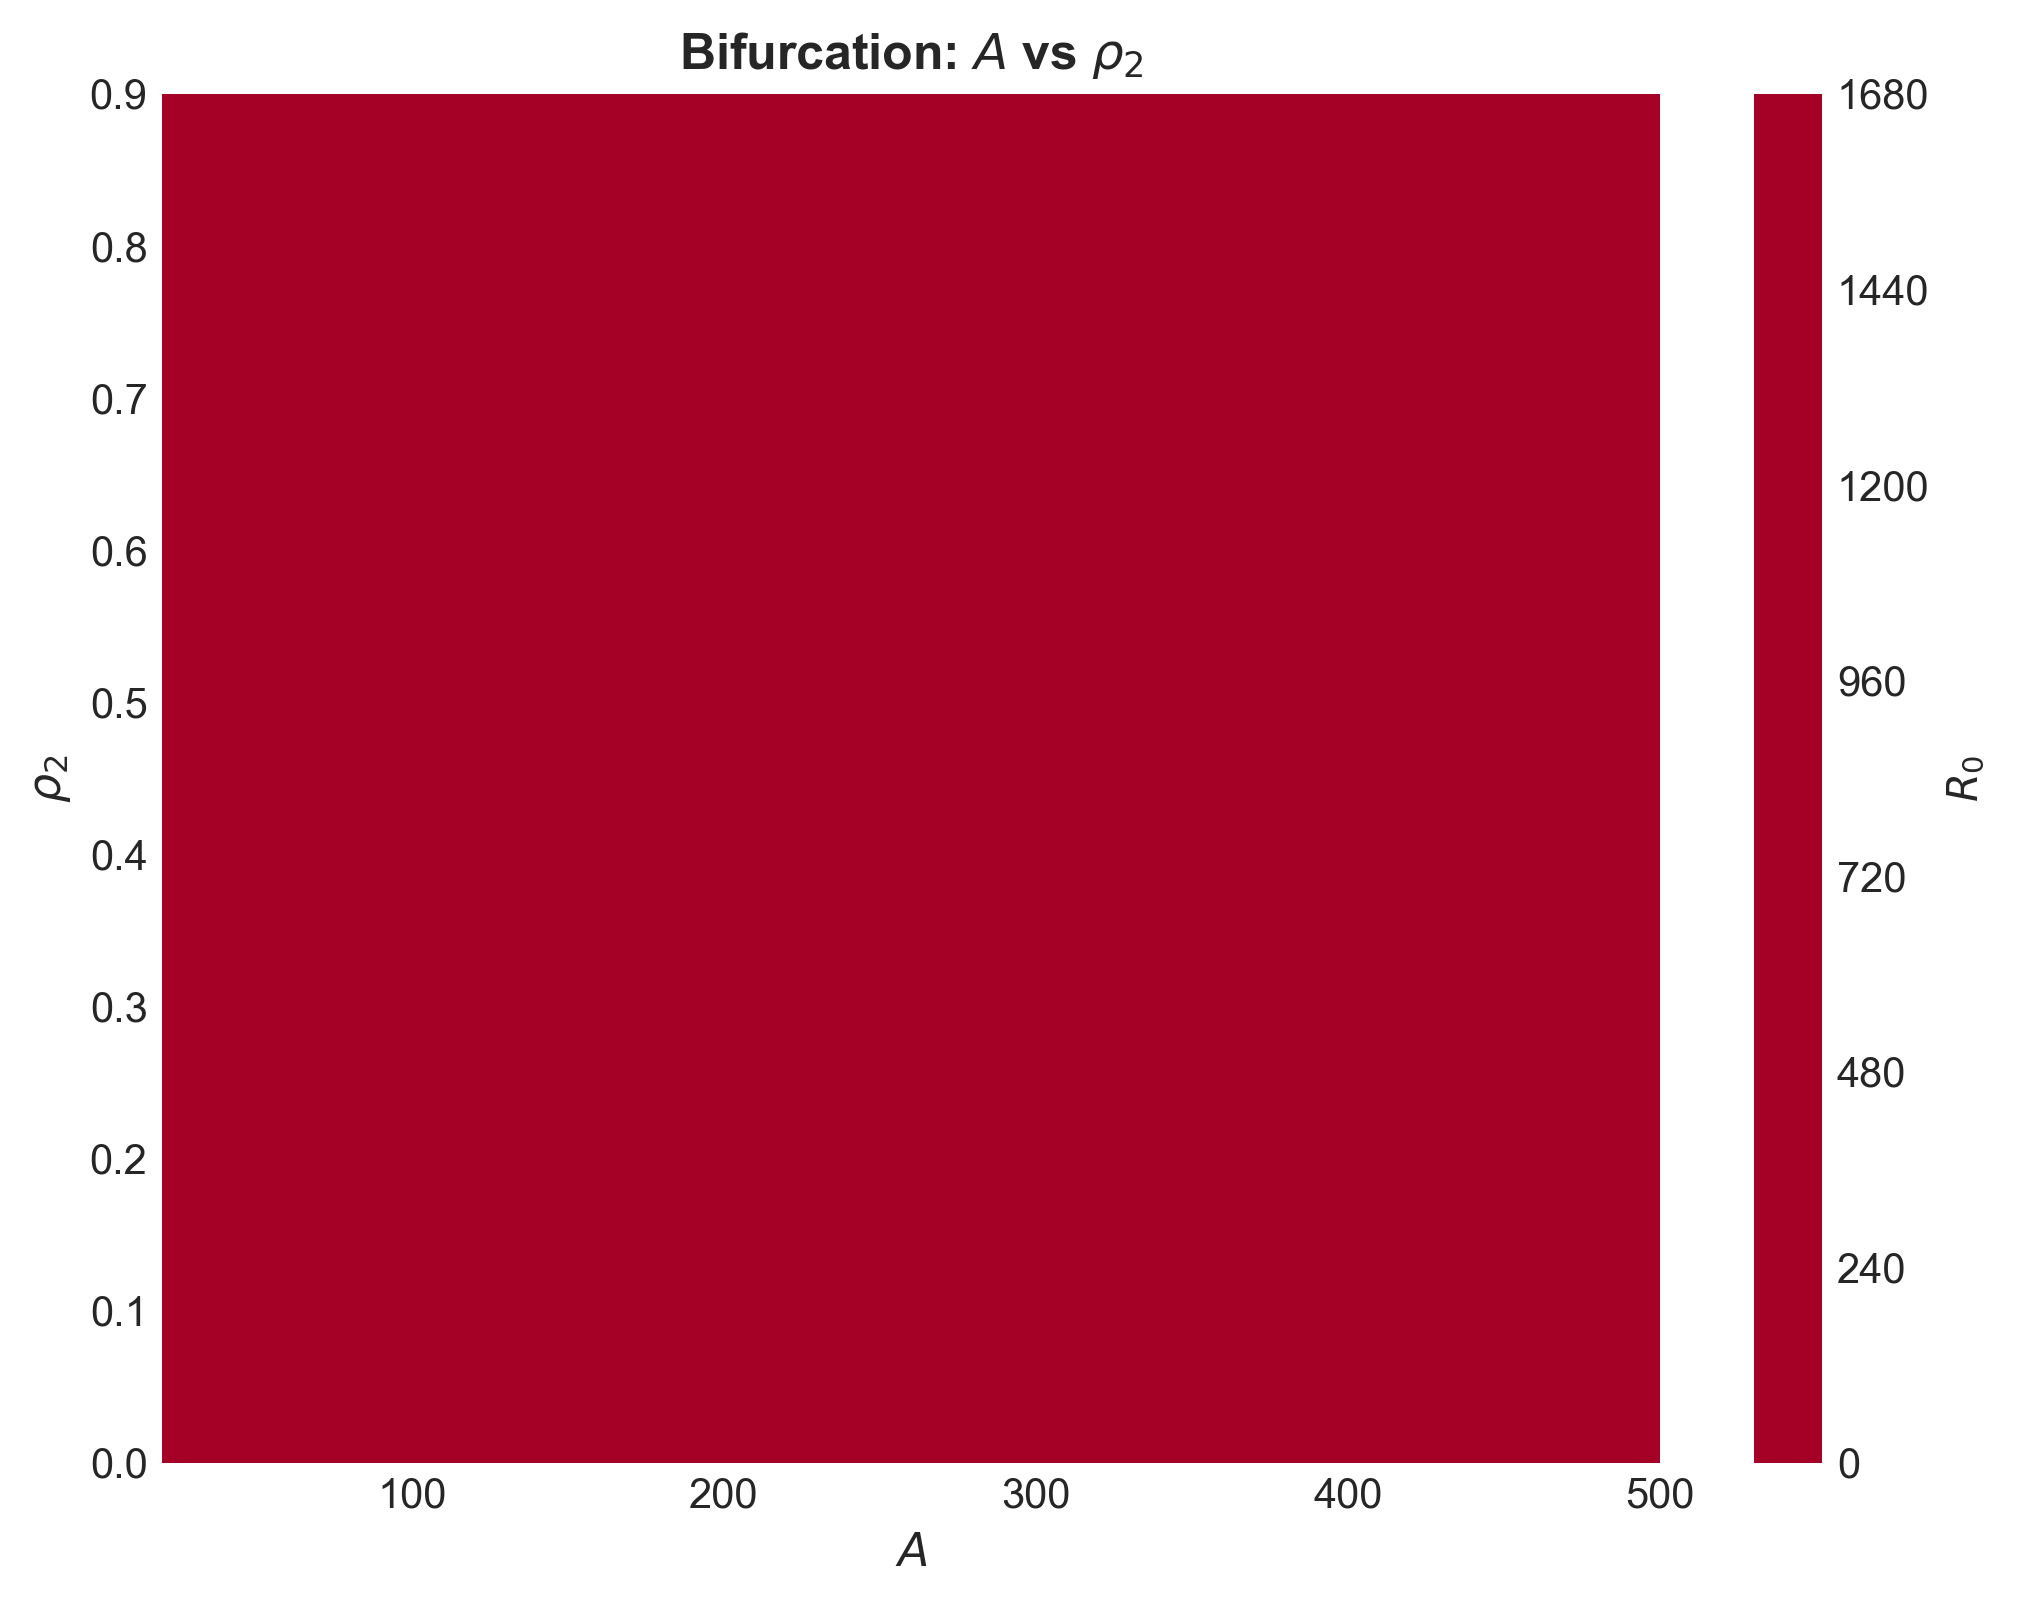
\includegraphics[width=0.55\linewidth]{A_vs_rho2onR.png}
    \caption{Bifurcation diagram in the $(A,\rho_2)$ plane highlighting the role of precautionary measures in disease control.}
    \label{fig:A_rho2}
\end{figure}

Figure~\ref{fig:A_rho1} illustrates the combined effect of recruitment rate $A$ and social distancing intensity $\rho_1$. Higher values of $\rho_1$ significantly reduce disease spread by lowering effective transmission, shifting the system toward the disease-free equilibrium. This result emphasizes the importance of social distancing policies in mitigating epidemic outbreaks under high population recruitment.

\begin{figure}[H]
    \centering
    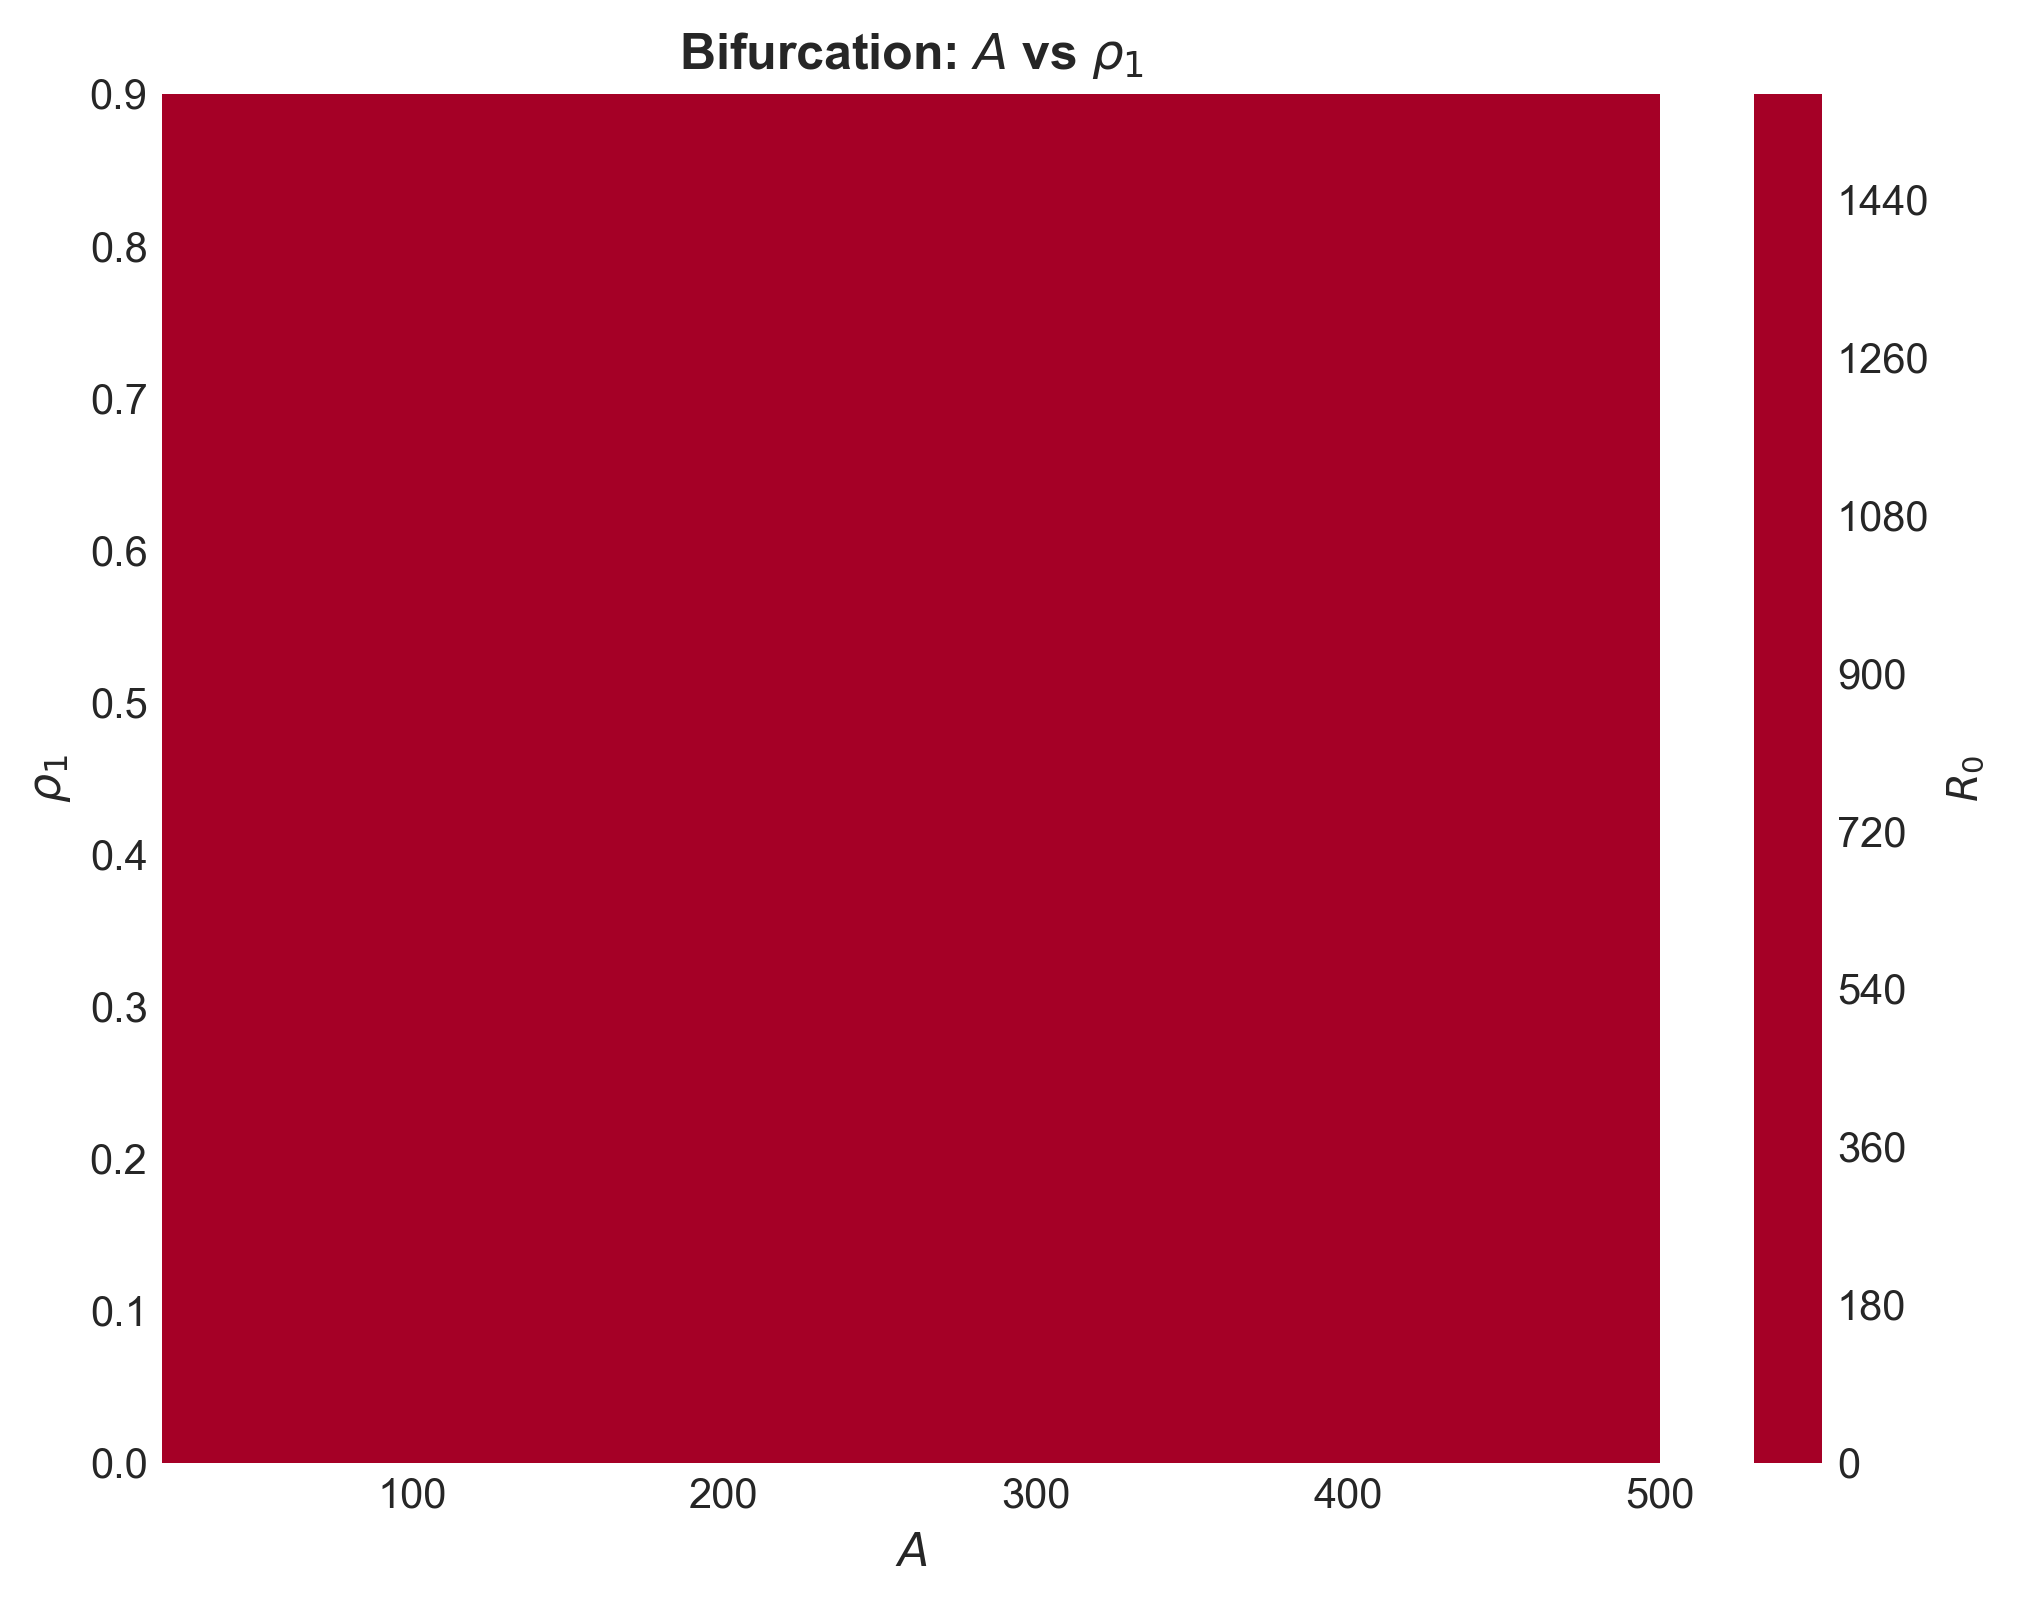
\includegraphics[width=0.55\linewidth]{A_vs_rho1onR.png}
    \caption{Two-parameter bifurcation diagram in the $(A,\rho_1)$ plane showing the stabilizing effect of social distancing.}
    \label{fig:A_rho1}
\end{figure}

The bifurcation diagram in Figure~\ref{fig:A_b1} represents the interaction between recruitment rate $A$ and the rate $b_1$ at which quarantined individuals return to the susceptible class. Higher values of $b_1$ may increase susceptibility within the population, promoting disease persistence. The threshold curve indicates that excessive release from quarantine can destabilize the disease-free equilibrium, particularly under high recruitment conditions.

\begin{figure}[H]
    \centering
    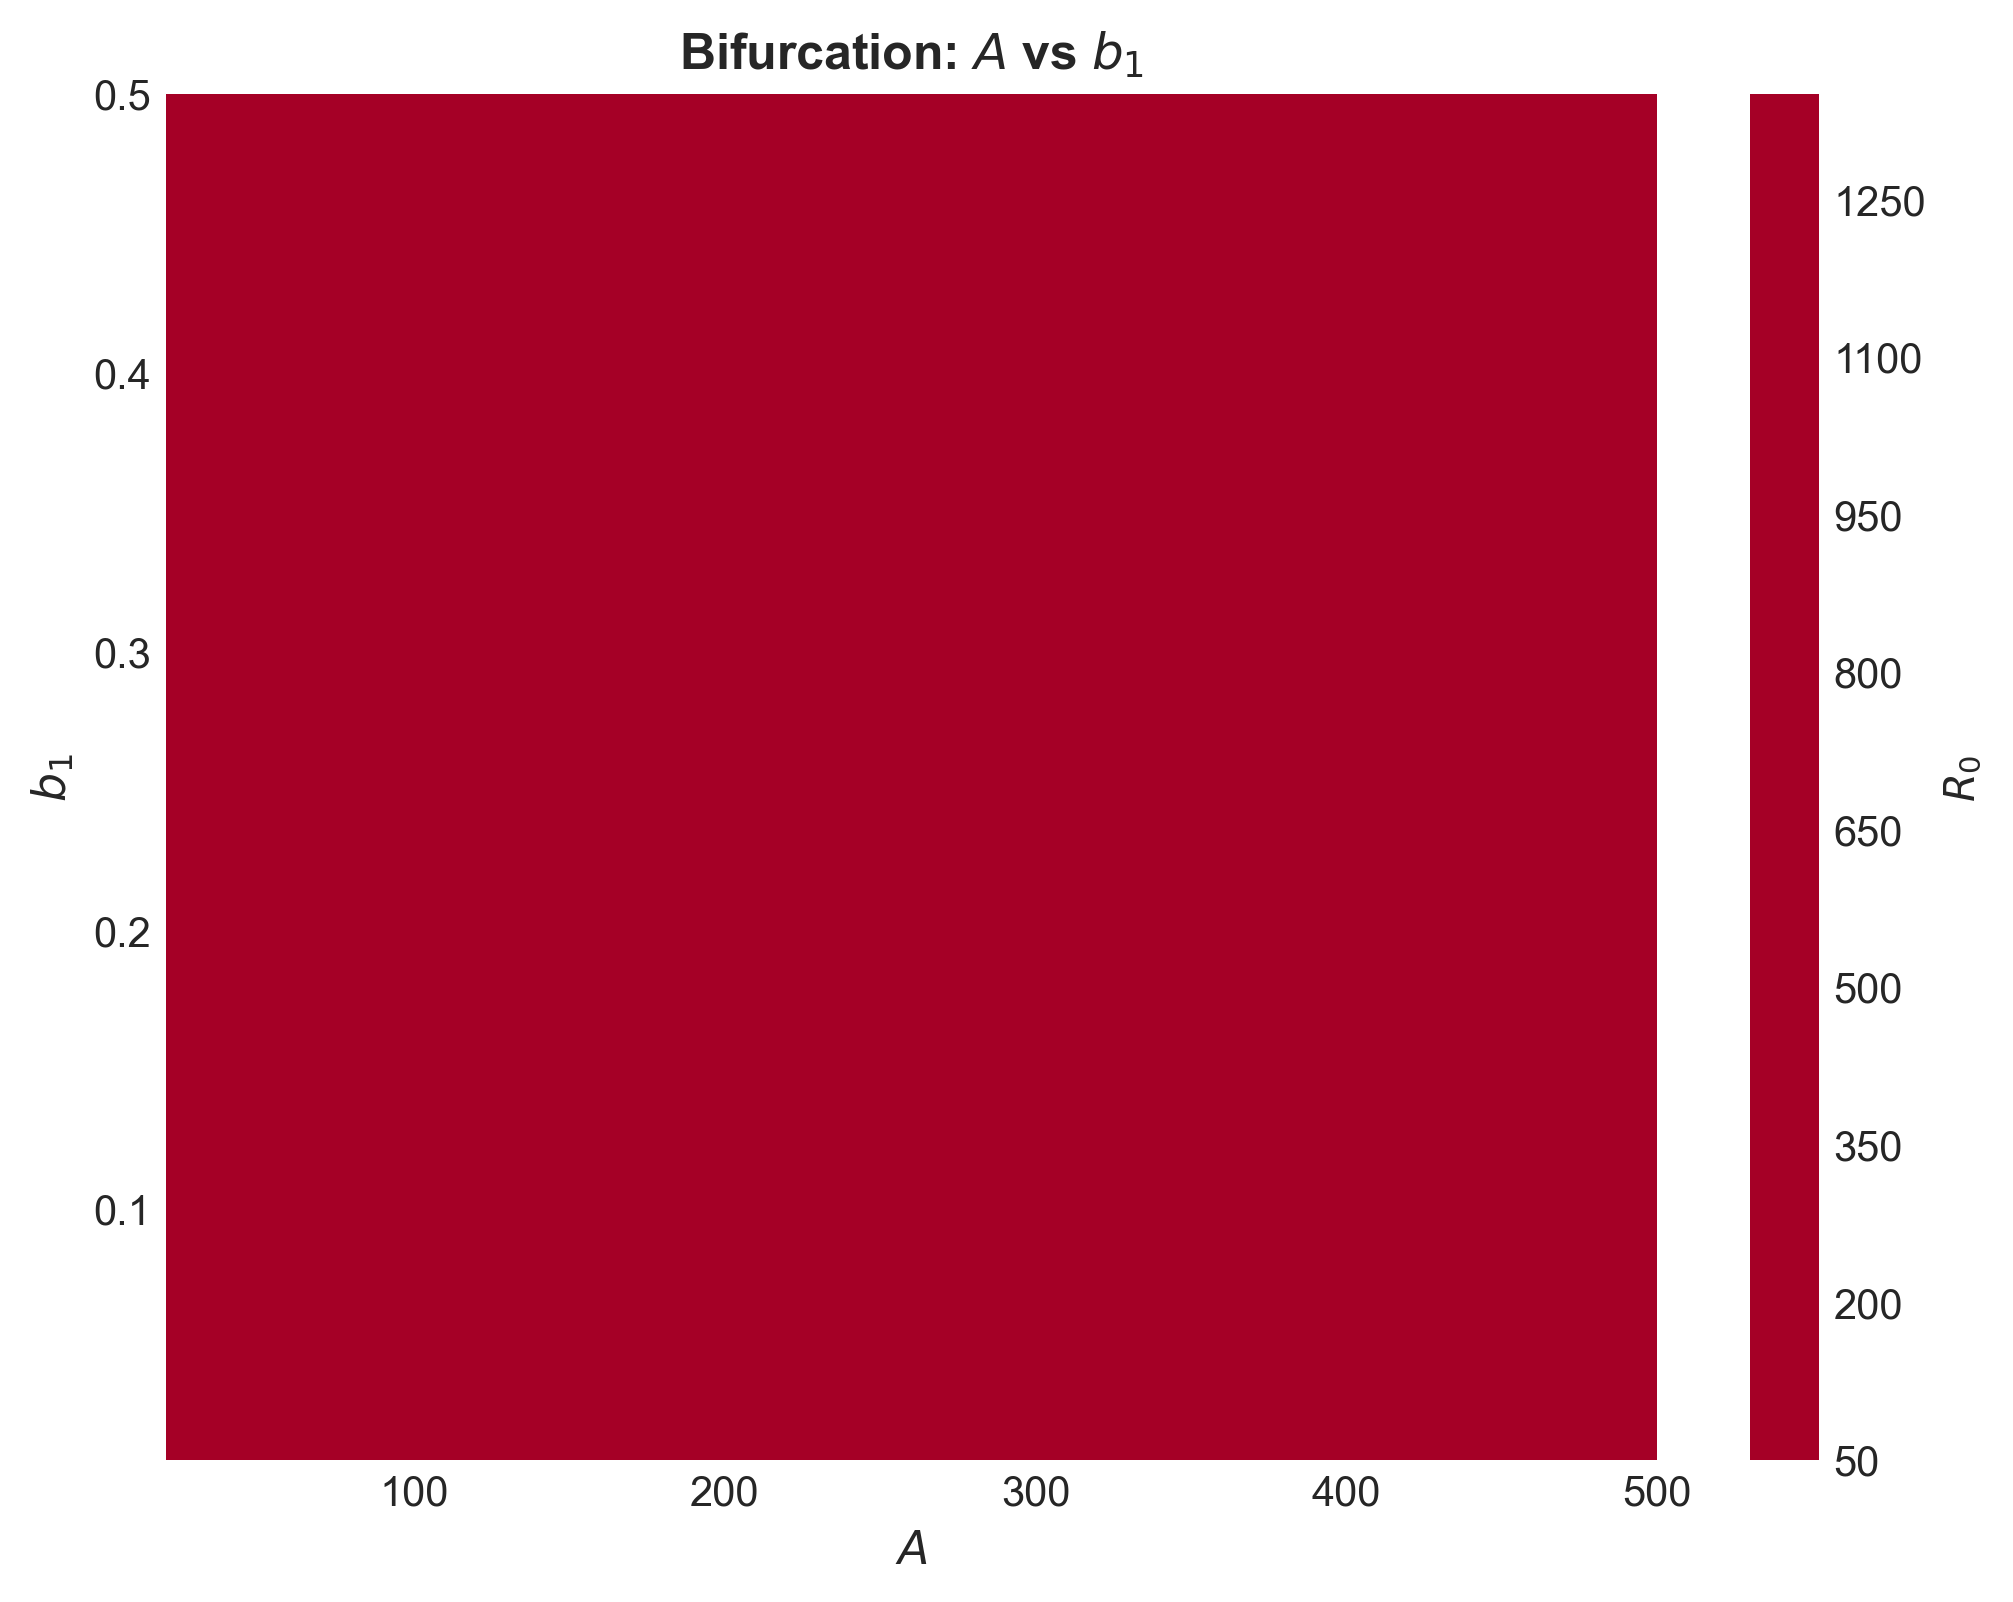
\includegraphics[width=0.55\linewidth]{A_vs_b1onR.png}
    \caption{Bifurcation diagram in the $(A,b_1)$ plane showing the effect of quarantine release on disease spread.}
    \label{fig:A_b1}
\end{figure}

Figure~\ref{fig:A_b2} illustrates the joint influence of recruitment rate $A$ and the quarantine rate $b_2$ of exposed individuals. Increasing $b_2$ effectively reduces the infectious pool by isolating exposed individuals, thereby suppressing disease transmission. The bifurcation boundary shows that efficient quarantine strategies can maintain disease-free stability even with high population recruitment.

\begin{figure}[H]
    \centering
    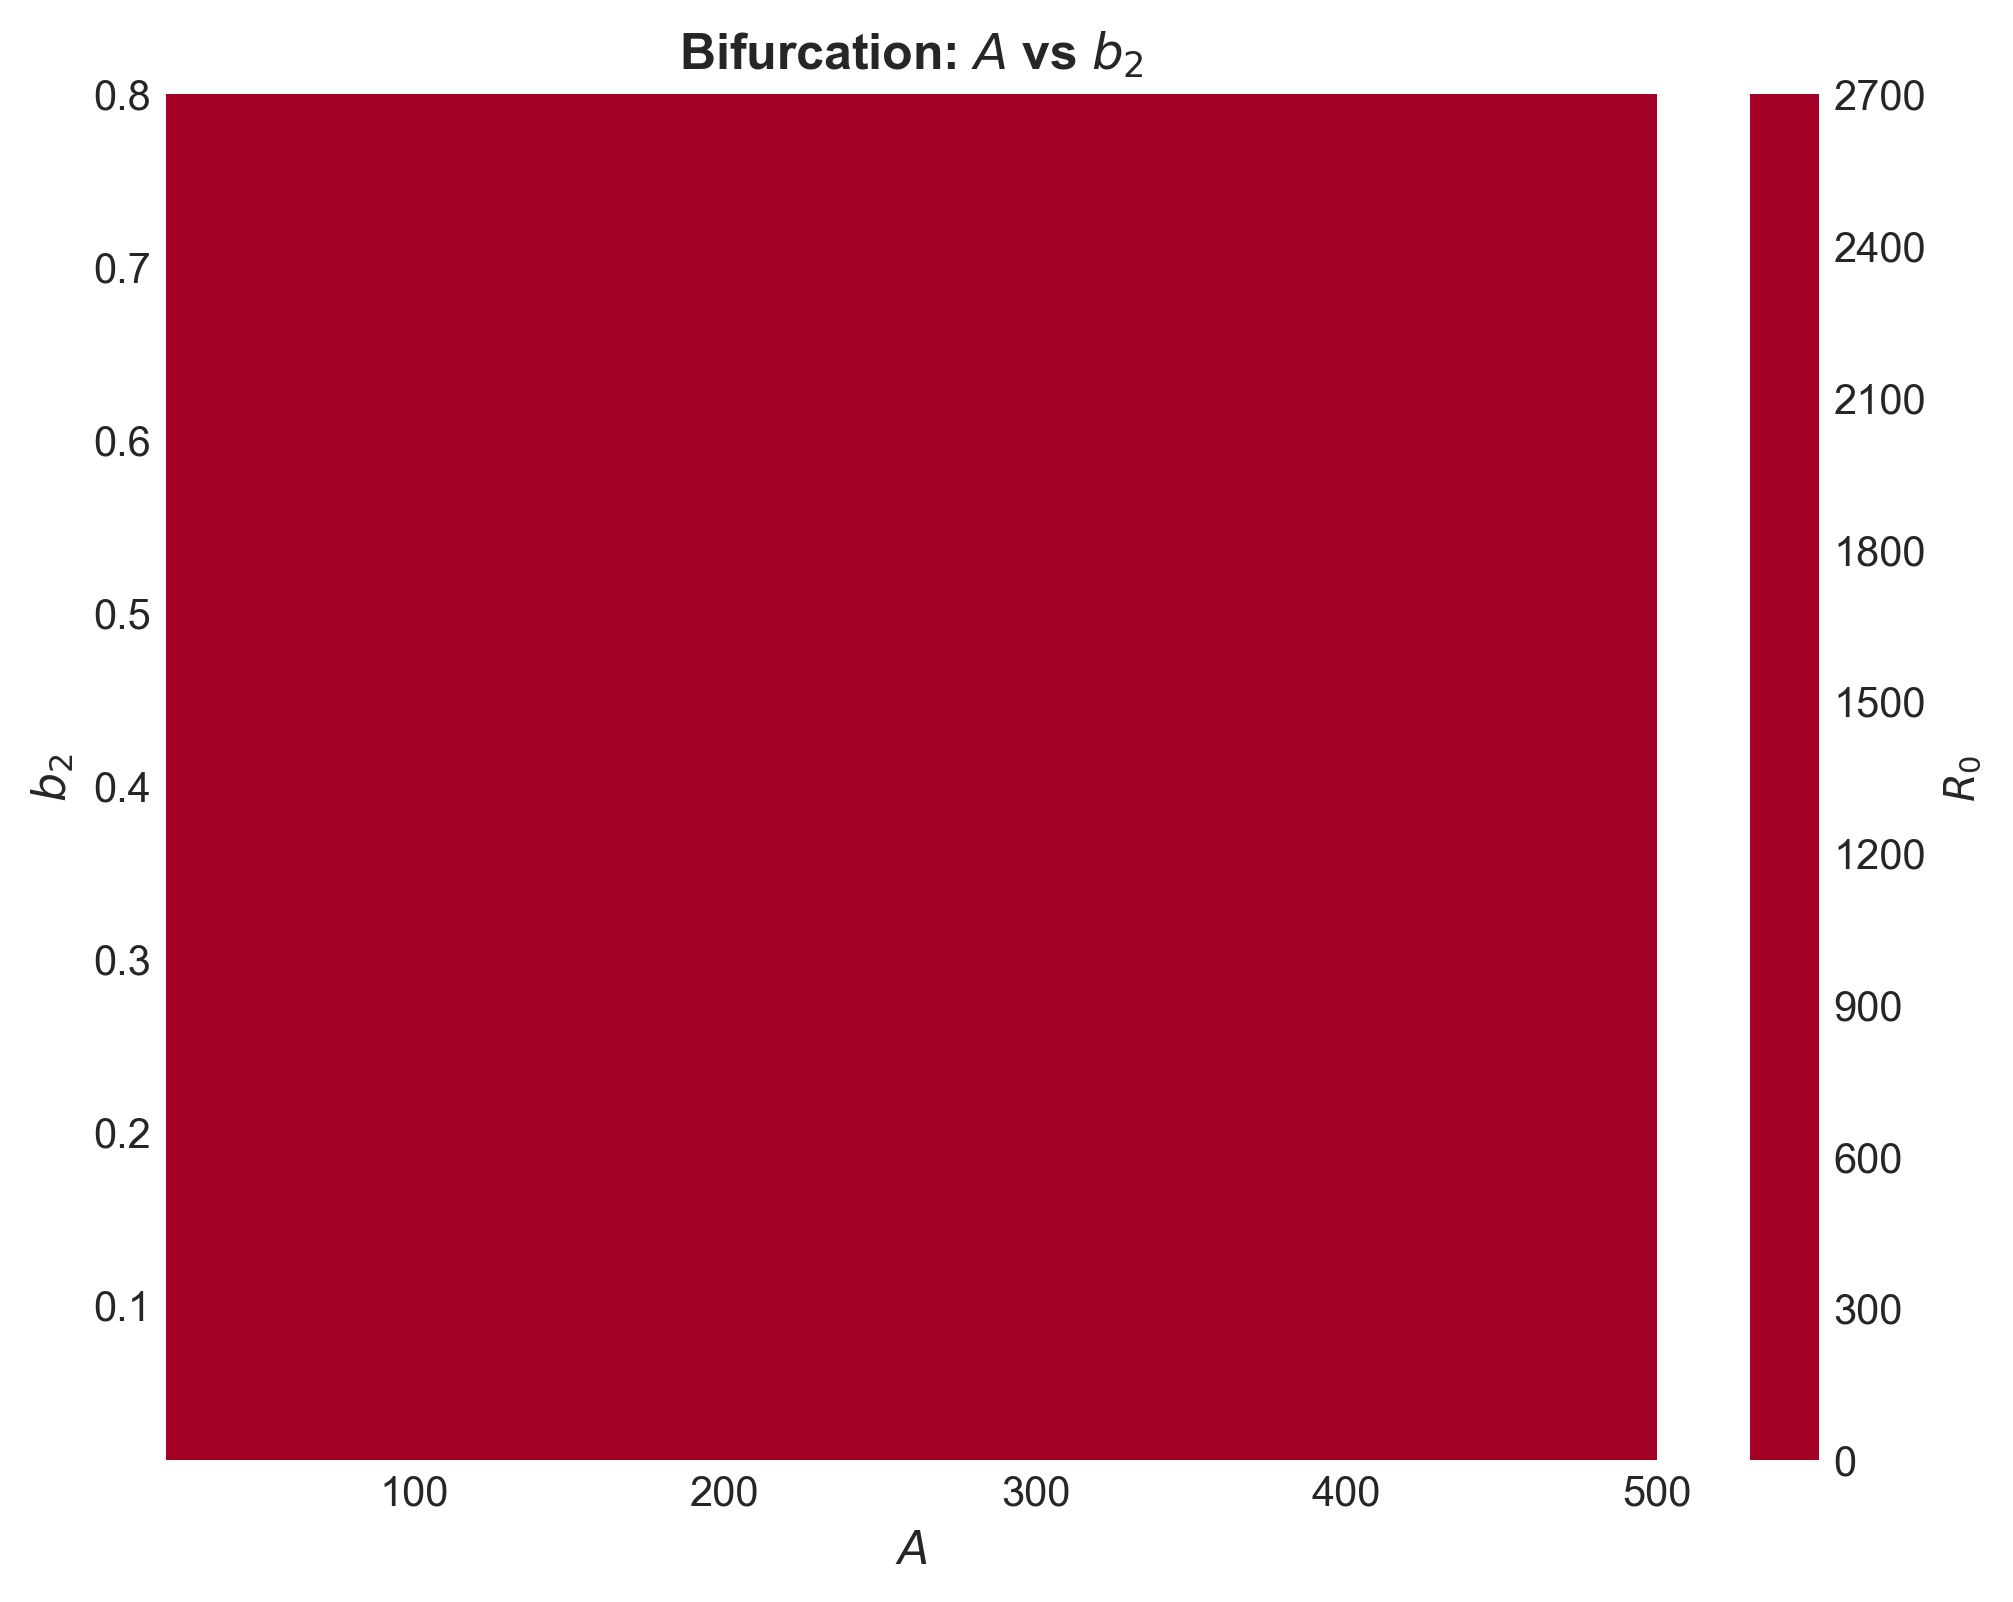
\includegraphics[width=0.55\linewidth]{A_vs_b2.png}
    \caption{Two-parameter bifurcation diagram in the $(A,b_2)$ plane highlighting the role of quarantine in epidemic control.}
    \label{fig:A_b2}
\end{figure}

Figure~\ref{fig:A_alpha} depicts the interaction between the recruitment rate $A$ and the infection progression rate $\alpha$. Higher values of $\alpha$ reduce the average latent period, leading to quicker isolation or recovery and lower transmission potential. The bifurcation curve highlights that faster disease progression can offset the destabilizing effect of increased recruitment.

\begin{figure}[H]
    \centering
    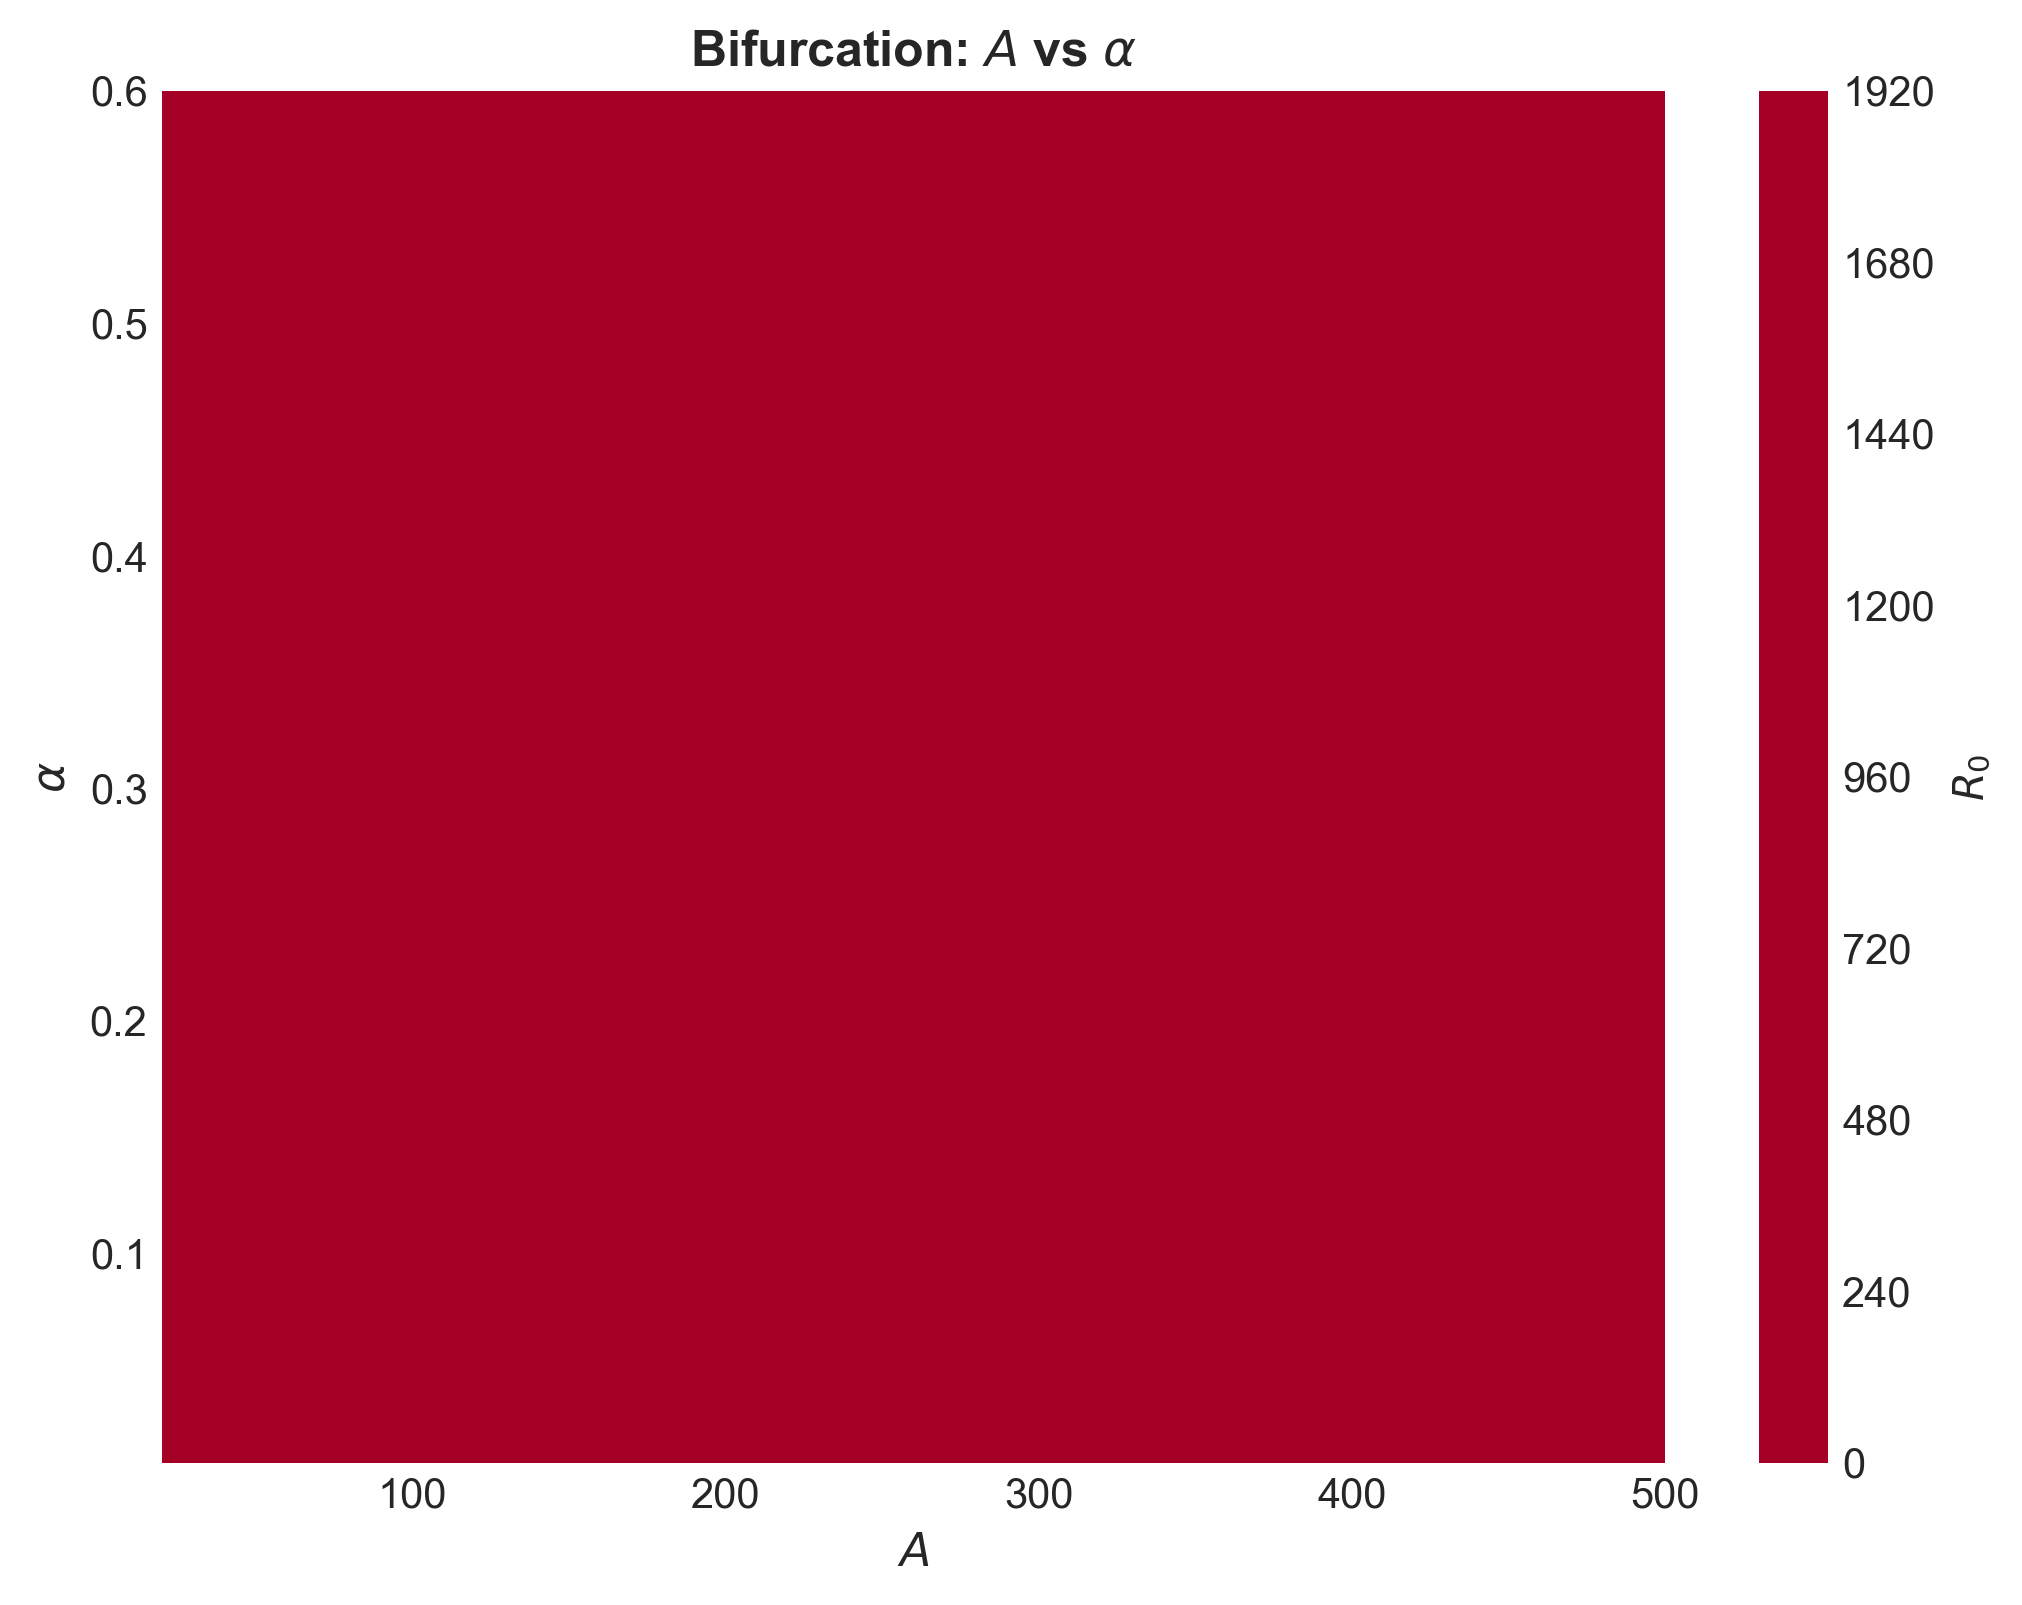
\includegraphics[width=0.55\linewidth]{A_vs_alphaonR.png}
    \caption{Bifurcation diagram in the $(A,\alpha)$ plane showing the effect of infection progression on disease dynamics.}
    \label{fig:A_alpha}
\end{figure}

The bifurcation diagram in Figure~\ref{fig:A_eta} illustrates the combined effect of recruitment rate $A$ and the recovery rate $\eta$. Increasing recovery reduces the infectious period and suppresses secondary infections. The threshold boundary indicates that effective treatment and recovery strategies play a crucial role in maintaining disease-free equilibrium under high recruitment scenarios.
\begin{figure}[H]
    \centering
    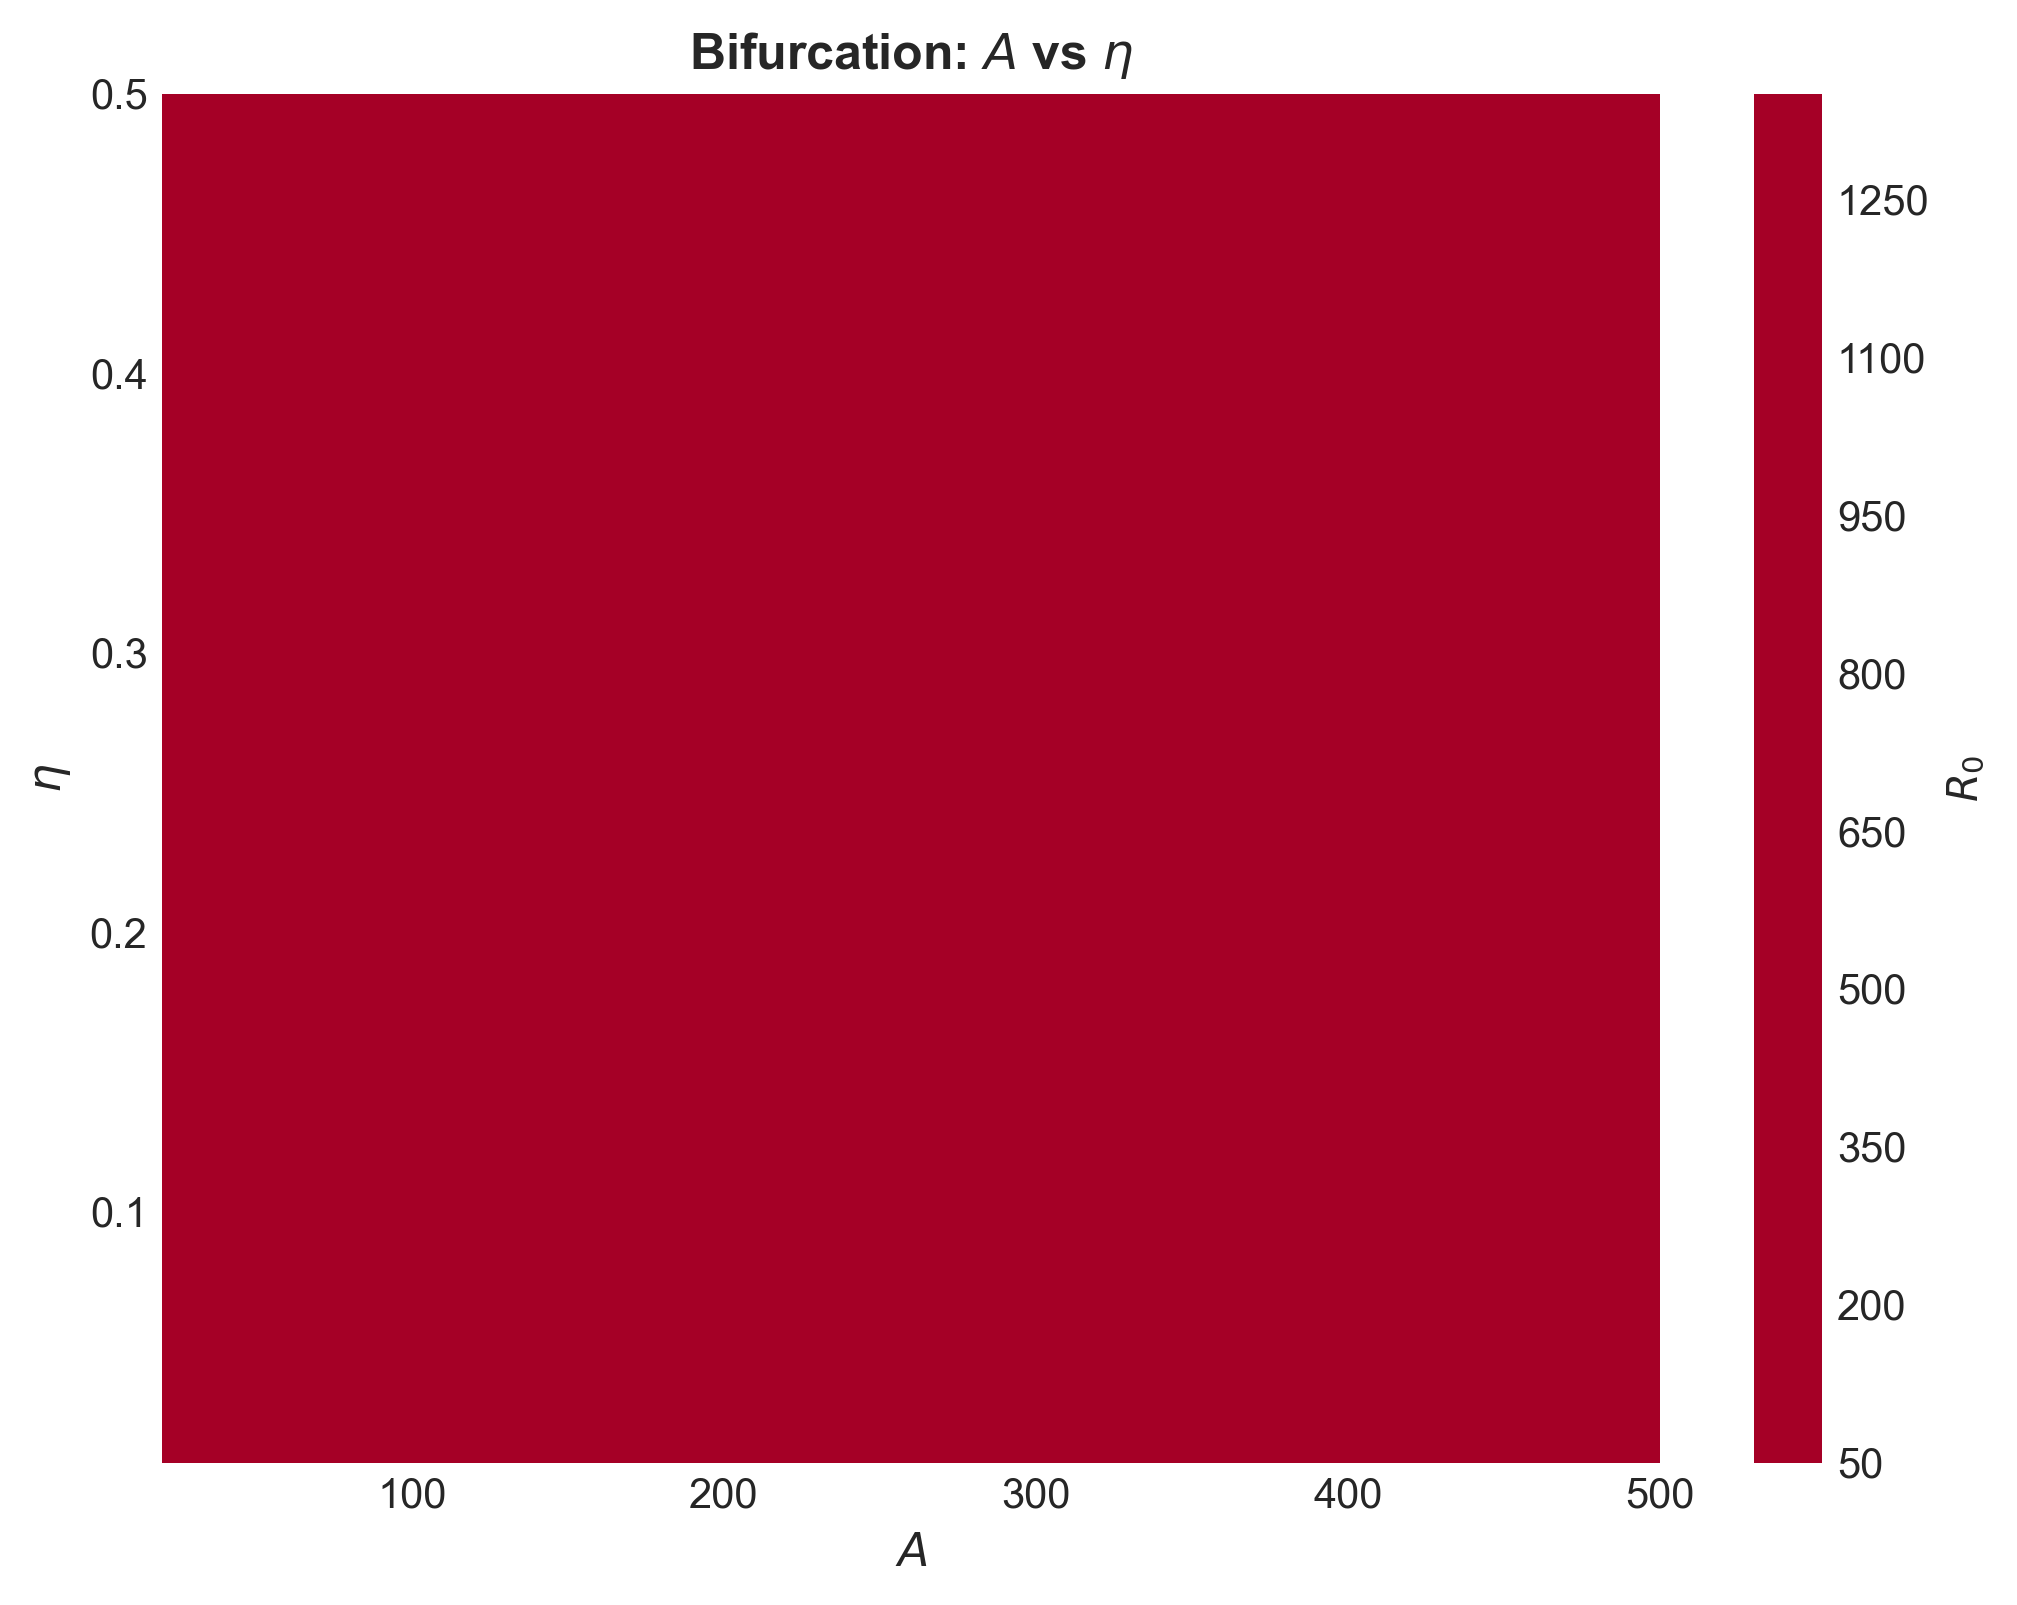
\includegraphics[width=0.55\linewidth]{A_vs_eta.png}
    \caption{Two-parameter bifurcation diagram in the $(A,\eta)$ plane showing the impact of recovery on disease control.}
    \label{fig:A_eta}
\end{figure}

Figure~\ref{fig:A_c} represents the interaction between the recruitment rate $A$ and the transition rate $c$ from quarantine to the infected class. Higher values of $c$ increase disease transmission by accelerating the movement of individuals into the infected compartment. The bifurcation boundary highlights the importance of controlling infection leakage from quarantine facilities to prevent endemic persistence.

\begin{figure}[H]
    \centering
    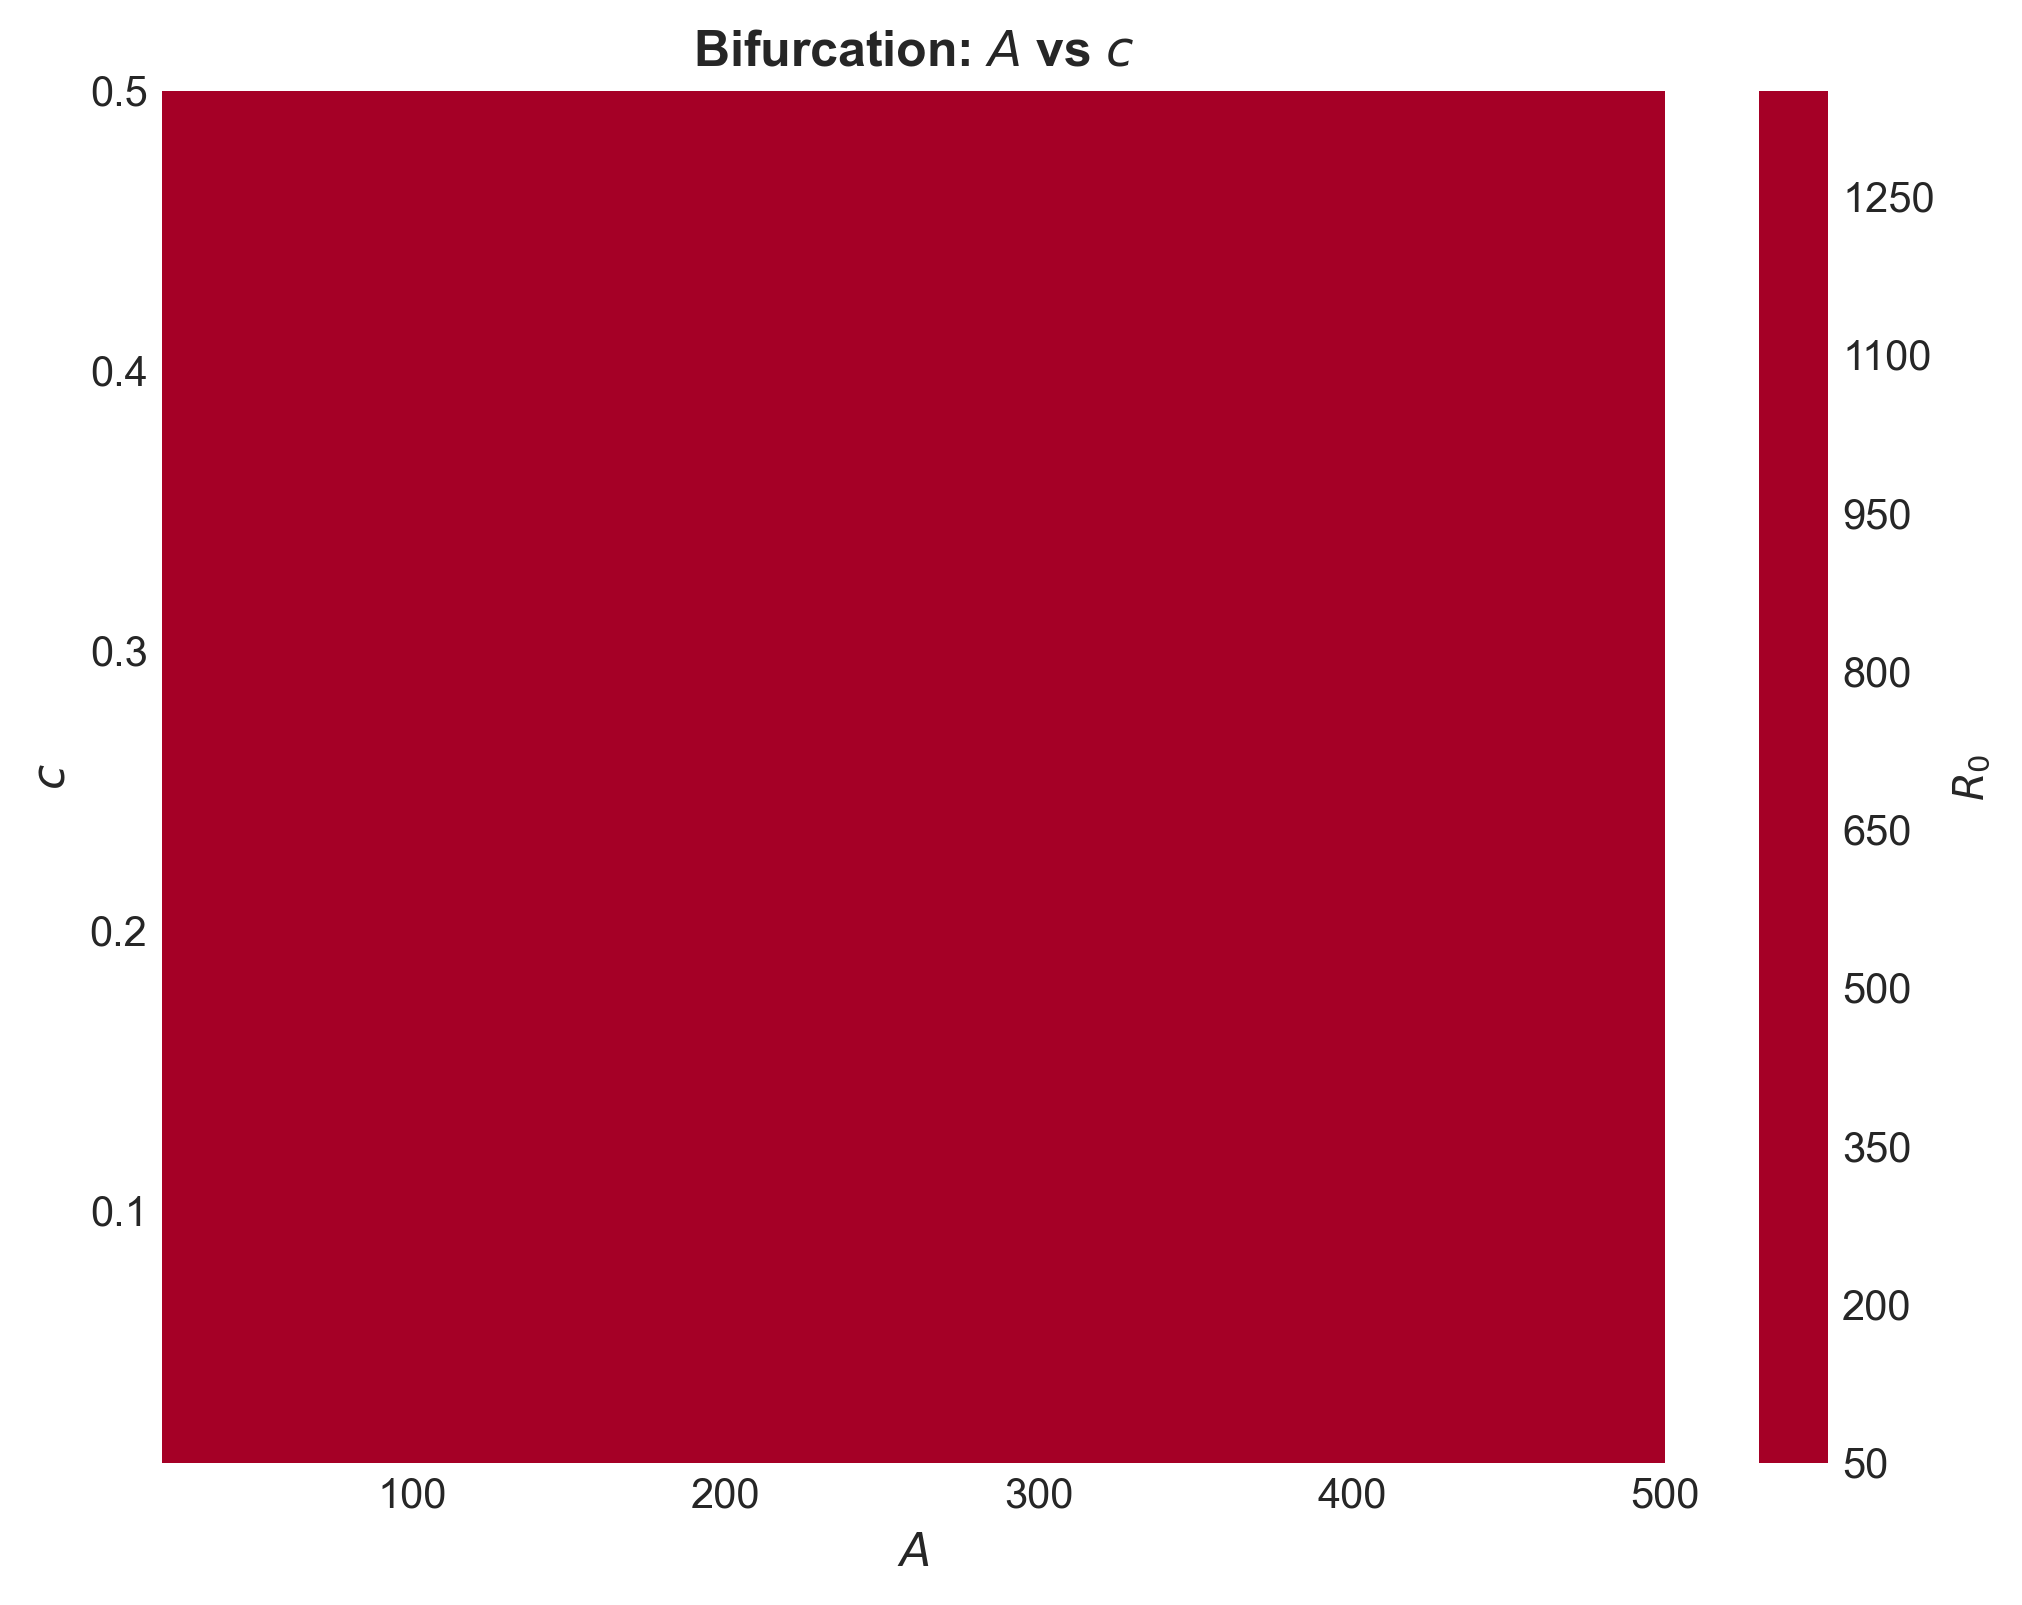
\includegraphics[width=0.55\linewidth]{A_vs_conR.png}
    \caption{Bifurcation diagram in the $(A,c)$ plane illustrating the impact of quarantine leakage on epidemic spread.}
    \label{fig:A_c}
\end{figure}

\section{Global Sensitivity Analysis Using PRCC}

In this section, a global sensitivity analysis is performed to quantify the relative influence of model parameters on the basic reproduction number $R_0$. Partial Rank Correlation Coefficients (PRCCs) are computed using Latin hypercube-type random sampling across biologically feasible parameter ranges. PRCC measures the strength and direction of the monotonic relationship between each parameter and $R_0$, while controlling for the effects of all other parameters. Positive PRCC values indicate parameters that increase disease transmission when their values increase, whereas negative PRCC values correspond to control parameters that reduce $R_0$ and contribute to disease mitigation.

Figure~\ref{fig:prcc_R0} illustrates the global sensitivity indices of $R_0$ with respect to key epidemiological parameters. The transmission rate $\beta$ and recruitment rate $A$ exhibit strong positive PRCC values, indicating that increases in these parameters significantly amplify disease spread. In contrast, the protection-related parameters $\rho_1$ and $\rho_2$ show strong negative correlations with $R_0$, highlighting the effectiveness of social distancing and precautionary measures in suppressing transmission. Additionally, the quarantine rate $b_2$, progression rate $\alpha$, and immunity-related parameter $\sigma$ display negative sensitivities, emphasizing their role in reducing secondary infections. Parameters with larger absolute PRCC values exert a greater influence on $R_0$, identifying $\beta$, $\rho_2$, and $\rho_1$ as the most dominant drivers of disease dynamics in the proposed model.

\begin{figure}[H]
    \centering
    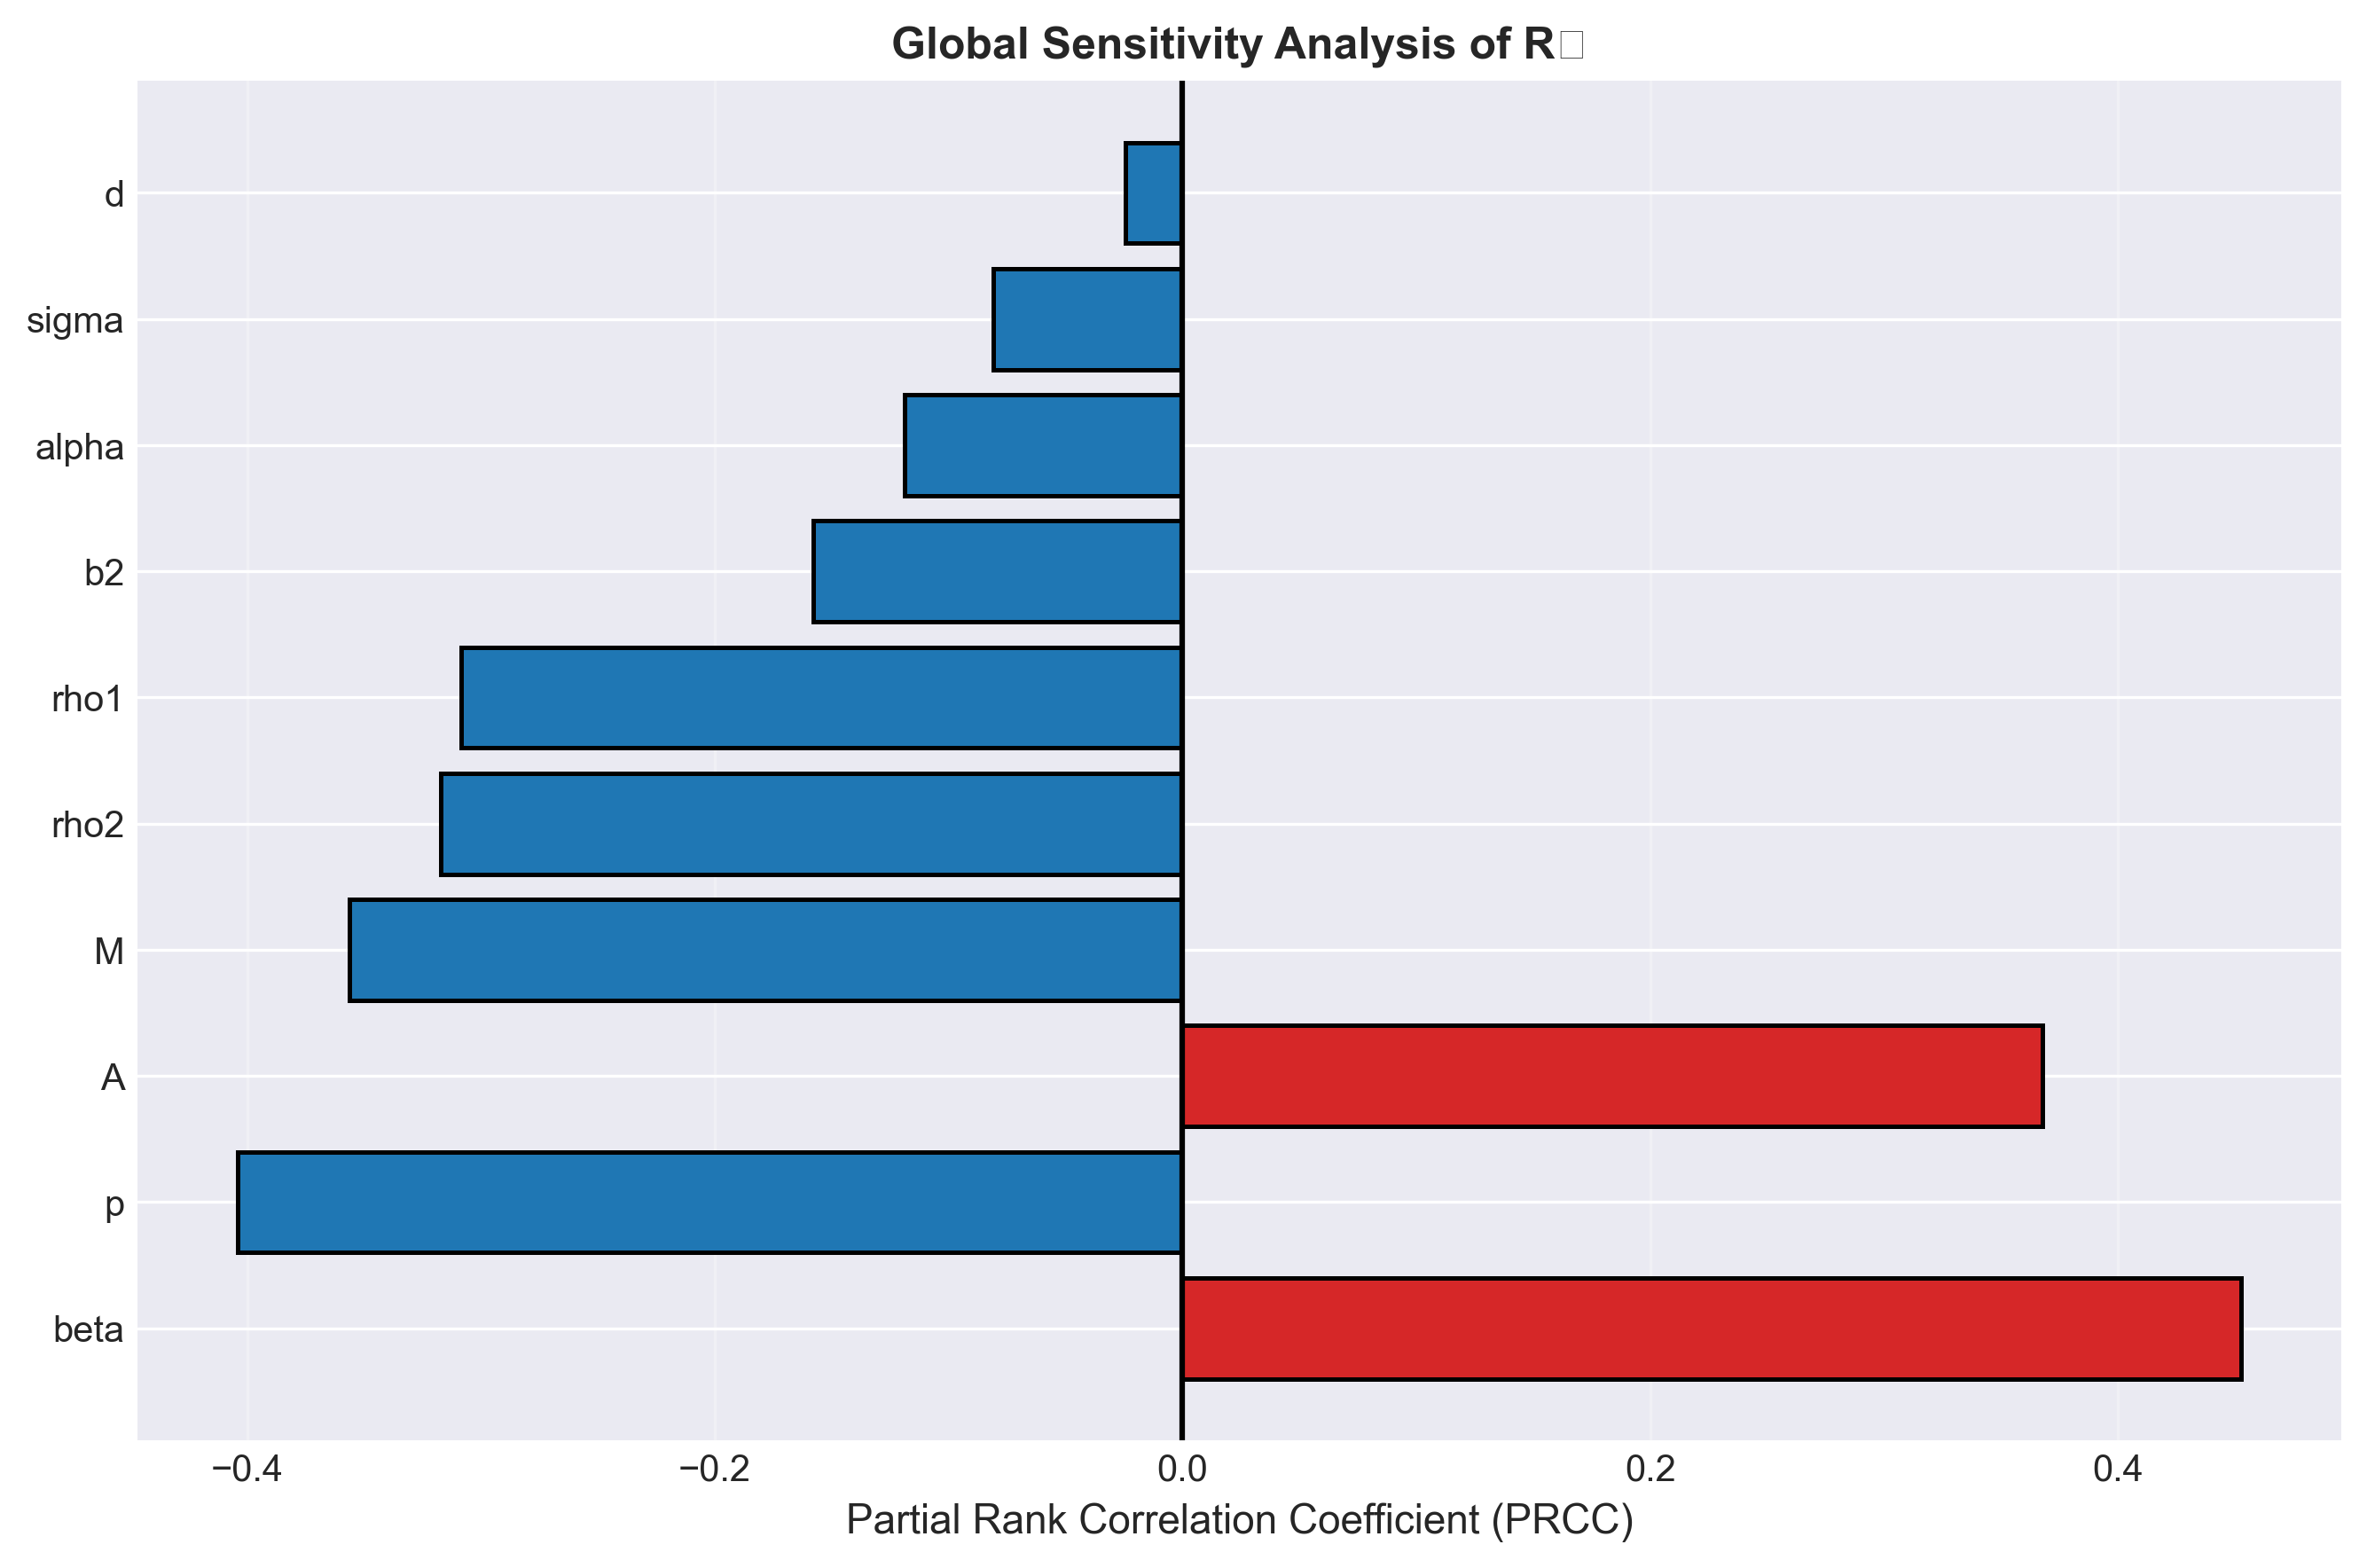
\includegraphics[width=0.85\linewidth]{PRCC_Sensitivity.png}
    \caption{Global sensitivity analysis of the basic reproduction number $R_0$ using Partial Rank Correlation Coefficients (PRCC). Positive values indicate parameters that enhance disease transmission, while negative values correspond to parameters contributing to disease control.}
    \label{fig:prcc_R0}
\end{figure}



\end{document}